\section{Resoconto delle attività di verifica}
In seguito vengono presentati i resoconti delle attività di verifica svolte.
Questa sezione viene mantenuta in costante aggiornamento rispetto alle revisioni di avanzamento del progetto\glo.
\subsection{Revisione dei requisiti (RR)}
\subsubsection{Analisi statica dei documenti}
L'analisi statica\glosp dei documenti ha portato alla produzione di una lista degli errori comuni. Questa lista, che deve essere mantenuta aggiornata con le prossime analisi, andrà a facilitare il compito dei verificatori.
\subsubsection{Esiti delle verifiche}
\paragraph{Qualità di prodotto}
\paragraph*{PRD-Q1 Documenti}
\subparagraph*{M15 Indice di Gulpease}\mbox{} %mbox perché altrimenti il paragraph finisce sotto al contenuto
%\subparagraph{Revisione dei Requisiti} \mbox{}
\begin{longtable} {						
		>{}p{50mm}  		
		>{}p{8mm}		
		>{}p{8mm}		
		>{}p{8mm}		
		>{}p{8mm}		
		>{}p{8mm}		
		>{}p{8mm}
		>{}p{8mm}
		>{}p{8mm}
		>{}p{8mm}				
	}			
	\rowcolor{gray!50}
	\textbf{Documento} & \textbf{I} & \textbf{II} & \textbf{III} & \textbf{IV} & \textbf{V} & \textbf{VI} \TBstrut \\ [2mm]
	\textbf{Analisi dei Requisiti} & 80 & 83 & 89 & 75 & 82 & 82 \TBstrut \\ [2mm]
	\textbf{Studio di Fattibilità} & 95 & 94 & 98 & 97 & 96 & 100 \TBstrut \\ [2mm]
	\textbf{Norme di Progetto} & 43 & 54 & 57 & 58 & 60 & 63 \TBstrut \\ [2mm]
	\textbf{Piano di Progetto} & 65 & 68 & 63 & 62 & 60 & 63 \TBstrut \\ [2mm]
	\textbf{Piano di Qualifica} & 65 & 67 & 69 & 65 & 69 & 71 \TBstrut \\ [2mm]
	\textbf{Glossario} & 62 & 55 & 59 & 45 & 50 & 58 \TBstrut \\ [2mm]
	\textbf{Verbali interni (media)} & 87 & 85 & 84 & 83 & 82 & 78 \TBstrut \\ [2mm]
	\textbf{Verbali esterni (media)} & - & - & 62 & 62 & 61 & 61 \TBstrut \\ [2mm]
	\rowcolor{white}
	\caption{M15 revisione dei requisiti}
\end{longtable}
\begin{figure}[H] 	
	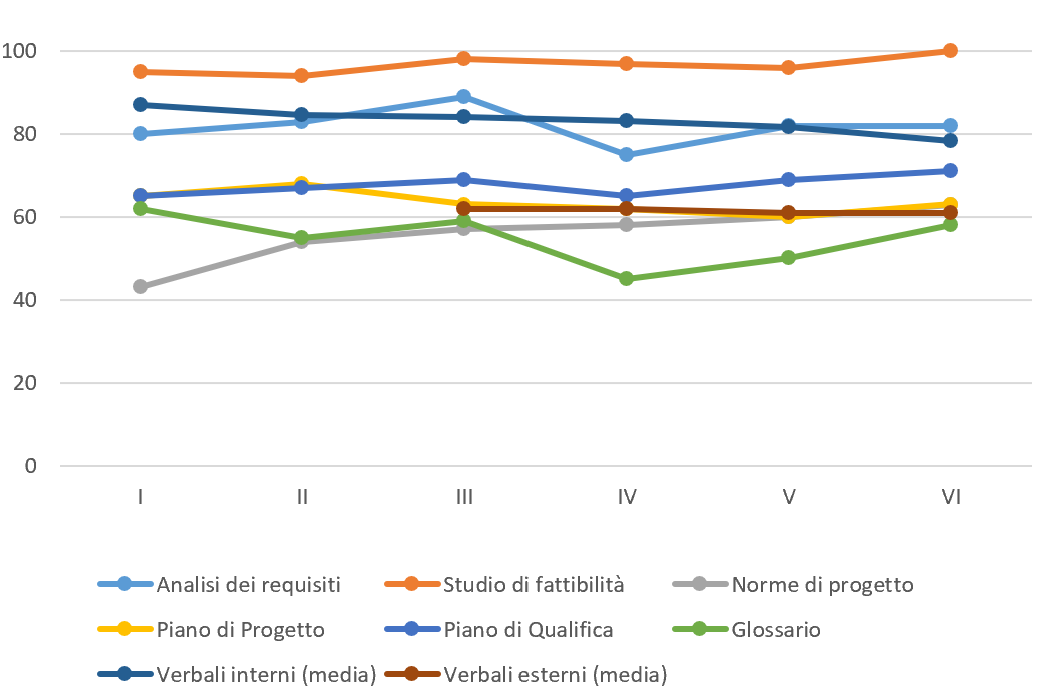
\includegraphics[width=\linewidth]{./img/grafici/2.png}	
	\caption{M15 revisione dei requisiti}	
\end{figure}
\subsubsection{Esito della revisione esterna}
Il gruppo ritiene poco soddisfacenti i risultati della revisione esterna. 
Le correzioni comunicate attraverso colloqui con i committenti e commenti alla valutazione ci hanno permesso di riflettere sui cambiamenti necessari da mettere in atto sia sui nostri prodotti che sul nostro way of working\glo.
Abbiamo quindi deciso di dare più importanza ai ruoli di verificatore e progettista per non ripetere gli errori della precedente revisione e per sopperire alle carenze segnalate.
Questo non si rifletterà con un aumento delle ore nei ruoli individuati, ma con un maggiore impegno da parte dei componenti del gruppo perché migliori la qualità delle ore svolte e non il numero.

\subsection{Revisione di progettazione (RP)}
\subsubsection{Riassunto delle attività di verifica}
In questo periodo abbiamo attuato le verifiche sui documenti, come nel precedente periodo. A queste abbiamo aggiunto le prime verifiche sulla codifica e sulla pianificazione per verificare che lo svolgimento del progetto\glosp procedesse senza impedimenti.  
\paragraph{Analisi statica dei documenti}
L'analisi statica\glosp dei documenti ha portato alla produzione di una lista degli errori comuni ridotti rispetto alla revisione precedente. Questa lista deve essere aggiornata con le prossime analisi e andrà a facilitare il compito dei verificatori.
\subsubsection{Esiti delle verifiche}
\paragraph{Qualità di processo}
\paragraph*{PRC-Q1 Processo di sviluppo}
\subparagraph{M01 Scostamento dei requisiti individuati} \mbox{}
\begin{longtable}[H!] {						
		>{}p{50mm}  		
		>{}p{8mm}
		>{}p{8mm}		
		>{}p{8mm}		
		>{}p{8mm}		
		>{}p{8mm}		
		>{}p{8mm}
		>{}p{8mm}
		>{}p{8mm}
		>{}p{8mm}
	}
\rowcolor{gray!50}
\textbf{} & \textbf{I} & \textbf{II} & \textbf{III} & \textbf{IV} & \textbf{V} \TBstrut \\ [2mm]
\textbf{Scostamenti} & 10 & 23 & 29 & 29 & 29 \TBstrut \\ [2mm]
	\rowcolor{white}
\caption{M01 revisione di progettazione\glo}
\end{longtable}
\begin{figure}[H] 	
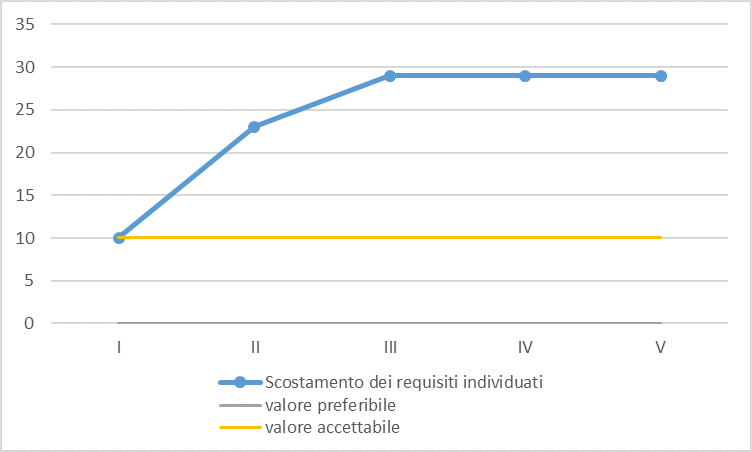
\includegraphics[width=\linewidth]{./img/grafici/RP1.png}	
\caption{M01 revisione di progettazione\glo}	
\end{figure}
\begin{itemize}
	\item \textbf{Valore preferibile}: 0;
	\item \textbf{Valore accettabile}: 10;
	\item \textbf{Considerazioni}: la metrica\glosp non risulta soddisfatta al termine del periodo di progettazione\glo.
\end{itemize}
\subparagraph{M02 Numero di parametri per metodo} \mbox{}
\begin{longtable}[H!] {						
		>{}p{50mm}  		
		>{}p{8mm}
		>{}p{8mm}		
		>{}p{8mm}		
		>{}p{8mm}		
		>{}p{8mm}		
		>{}p{8mm}
		>{}p{8mm}
		>{}p{8mm}
		>{}p{8mm}
	}
	\rowcolor{gray!50}
	\textbf{} & \textbf{I} & \textbf{II} & \textbf{III} & \textbf{IV} & \textbf{V} \TBstrut \\ [2mm]
	\textbf{Numero di parametri} & - & - & 3 & 3 & 4 \TBstrut \\ [2mm]
	\rowcolor{white}
	\caption{M02 revisione di progettazione\glo}
\end{longtable}
\begin{figure}[H] 	
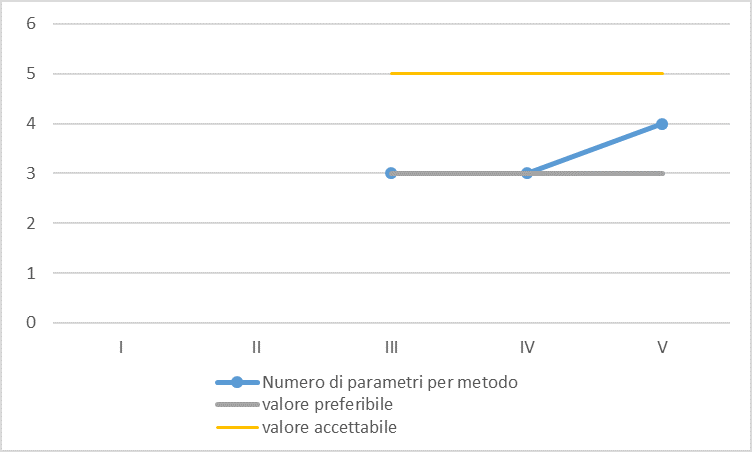
\includegraphics[width=\linewidth]{./img/grafici/RP2.png}	
\caption{M02 revisione di progettazione\glo}	
\end{figure}
\begin{itemize}
	\item \textbf{Valore preferibile}: $\le3$;
	\item \textbf{Valore accettabile}: $\le5$;
	\item \textbf{Considerazioni}: la metrica\glosp risulta soddisfatta al termine del periodo di progettazione\glo.
\end{itemize}
\pagebreak
\subparagraph{M03 Numero di metodi per classe} \mbox{}
\begin{longtable}[H!] {						
		>{}p{50mm}  		
		>{}p{8mm}
		>{}p{8mm}		
		>{}p{8mm}		
		>{}p{8mm}		
		>{}p{8mm}		
		>{}p{8mm}
		>{}p{8mm}
		>{}p{8mm}
		>{}p{8mm}
	}
	\rowcolor{gray!50}
	\textbf{} & \textbf{I} & \textbf{II} & \textbf{III} & \textbf{IV} & \textbf{V} \TBstrut \\ [2mm]
	\textbf{Numero di metodi} & - & - & 9 & 9 & 21 \TBstrut \\ [2mm]
	\rowcolor{white}
	\caption{M03 revisione di progettazione\glo}
\end{longtable}
\begin{figure}[H] 	
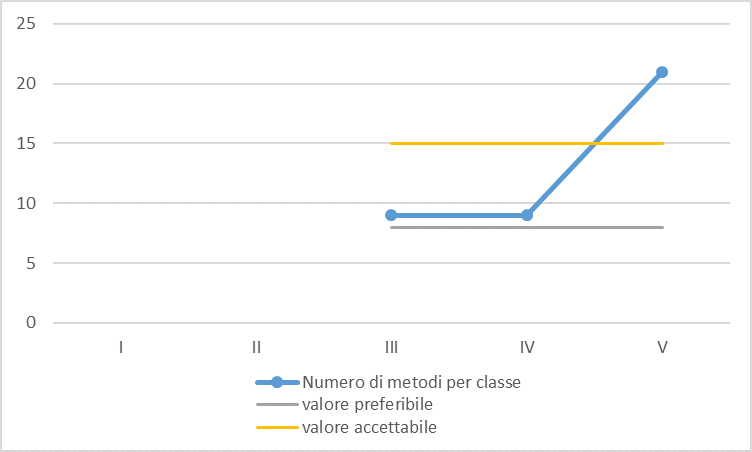
\includegraphics[width=\linewidth]{./img/grafici/RP3.png}	
\caption{M03 revisione di progettazione\glo}	
\end{figure}
\begin{itemize}
	\item \textbf{Valore preferibile}: $\le8$;
	\item \textbf{Valore accettabile}: $\le15$;
	\item \textbf{Considerazioni}: la metrica\glosp non risulta soddisfatta al termine del periodo di progettazione\glo.
\end{itemize}

\paragraph*{PRC-Q2 Processo di garanzia della qualità}
\subparagraph{M04 Percentuale di metriche soddisfatte} \mbox{}
\begin{longtable}[H!] {						
		>{}p{50mm}  		
		>{}p{8mm}
		>{}p{8mm}		
		>{}p{8mm}		
		>{}p{8mm}		
		>{}p{8mm}		
		>{}p{8mm}
		>{}p{8mm}
		>{}p{8mm}
		>{}p{8mm}
	}
	\rowcolor{gray!50}
	\textbf{} & \textbf{I} & \textbf{II} & \textbf{III} & \textbf{IV} & \textbf{V} \TBstrut \\ [2mm]
	\textbf{Percentuale} & 58\% & 33\% & 56\% & 72\% & 78\% \TBstrut \\ [2mm]
	\rowcolor{white}
	\caption{M04 revisione di progettazione\glo}
\end{longtable}
\begin{figure}[H] 	
	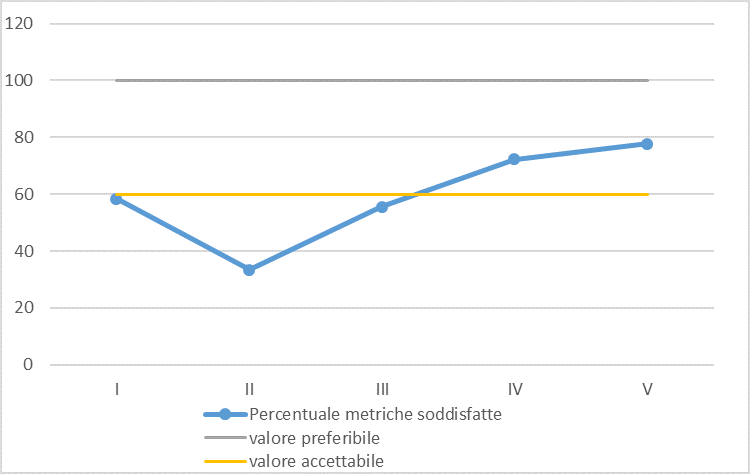
\includegraphics[width=\linewidth]{./img/grafici/RP19.png}	
	\caption{M04 revisione di progettazione\glo}	
\end{figure}
\begin{itemize}
	\item \textbf{Valore preferibile}: $=100\%$;
	\item \textbf{Valore accettabile}: $\ge60\%$;
	\item \textbf{Considerazioni}: la metrica\glosp risulta soddisfatta al termine del periodo di progettazione\glo.
\end{itemize}
\subparagraph{Considerazioni}
Il gruppo si ritiene soddisfatto rispetto al resoconto della verifica del periodo di progettazione architetturale visto il soddisfacimento della metrica M04. \\
Le metriche\glosp che non sono state soddisfatte al termine del V periodo sono le seguenti:
\begin{itemize}
	\item \textbf{M01 Scostamento dei requisiti individuati}: viene registrato uno spostamento significativo dei requisiti individuati, il gruppo ha lavorato per una comprendere in modo più approfondito le richieste del proponente per evitare che questo problema possa ripresentarsi in futuro;
	\item \textbf{M03 Numero di metodi per classe}: il prodotto\glosp dell'attività di codifica per l'implementazione del Proof of Concept\glosp non ha soddisfatto la soglia di accettabilità di questa metrica\glo. Perciò per il prossimo periodo analizzeremo le motivazioni di tale insuccesso per evitare che in futuro si ripresenti questo caso;
	\item \textbf{M16 Percentuale requisiti obbligatori soddisfatti}: il nostro prodotto\glo, come quindi anche il Proof of Concept\glo, viene realizzato in modo incrementale, perciò in questo periodo questa metrica\glosp non è ancora soddisfatta. Nei prossimi periodi abbiamo pianificato di lavorare con gli incrementi necessari a soddisfare i requisiti obbligatori mancanti;
	\item \textbf{M05 Percentuale bug sistemati}: il prodotto\glosp dell'attività di codifica per l'implementazione del Proof of Concept\glosp non ha rispettato questa metrica di qualità. Il gruppo ha deciso di analizzare assieme qual'è stato il problema per poterlo risolvere ed evitare che possa verificarsi nuovamente nei prossimi periodi.
\end{itemize}  

\paragraph*{PRC-Q3 Processo di verifica}
\subparagraph{M05 Percentuale bug sistemati} \mbox{}
\begin{longtable}[H!] {						
		>{}p{50mm}  		
		>{}p{8mm}
		>{}p{8mm}		
		>{}p{8mm}		
		>{}p{8mm}		
		>{}p{8mm}		
		>{}p{8mm}
		>{}p{8mm}
		>{}p{8mm}
		>{}p{8mm}
	}
	\rowcolor{gray!50}
	\textbf{} & \textbf{I} & \textbf{II} & \textbf{III} & \textbf{IV} & \textbf{V} \TBstrut \\ [2mm]
	\textbf{Bug sistemati} & - & - & 0\% & 30\% & 40\% \TBstrut \\ [2mm]
	\rowcolor{white}
	\caption{M05 revisione di progettazione\glo}
\end{longtable}
\begin{figure}[H] 	
	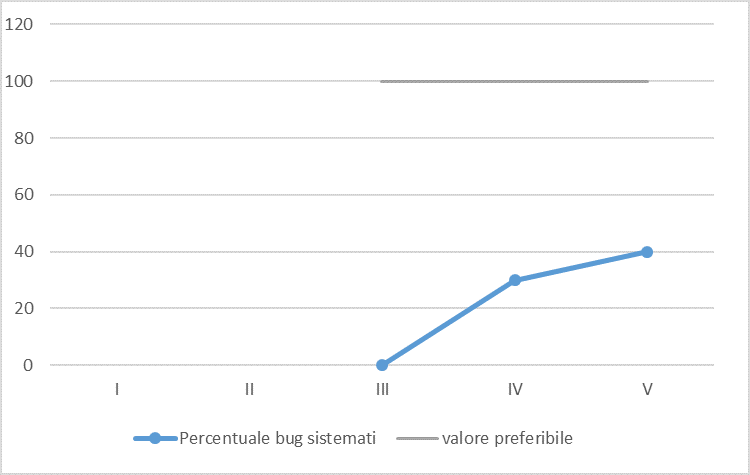
\includegraphics[width=\linewidth]{./img/grafici/RP16.png}	
	\caption{M05 revisione di progettazione\glo}	
\end{figure}
\begin{itemize}
	\item \textbf{Valore preferibile}: $=100\%$;
	\item \textbf{Valore accettabile}: $=100\%$;
	\item \textbf{Considerazioni}: la metrica\glosp risulta non soddisfatta al termine del periodo di progettazione\glo.
\end{itemize}

\paragraph*{PRC-Q4 Processo di gestione dei cambiamenti}
\subparagraph{M06 Tempo medio risoluzione errori} \mbox{}
\begin{longtable}[H!] {						
		>{}p{38mm}  		
		>{}p{12mm}
		>{}p{12mm}		
		>{}p{12mm}		
		>{}p{12mm}		
		>{}p{12mm}		
		>{}p{12mm}
		>{}p{12mm}
		>{}p{12mm}
		>{}p{12mm}
	}
	\rowcolor{gray!50}
	\textbf{} & \textbf{I} & \textbf{II} & \textbf{III} & \textbf{IV} & \textbf{V} \TBstrut \\ [2mm]
	\textbf{Tempo medio} & 15min & 134min & 122min & 110min & 104min \TBstrut \\ [2mm]
	\rowcolor{white}
	\caption{M06 revisione di progettazione\glo}
\end{longtable}
\begin{figure}[H] 	
	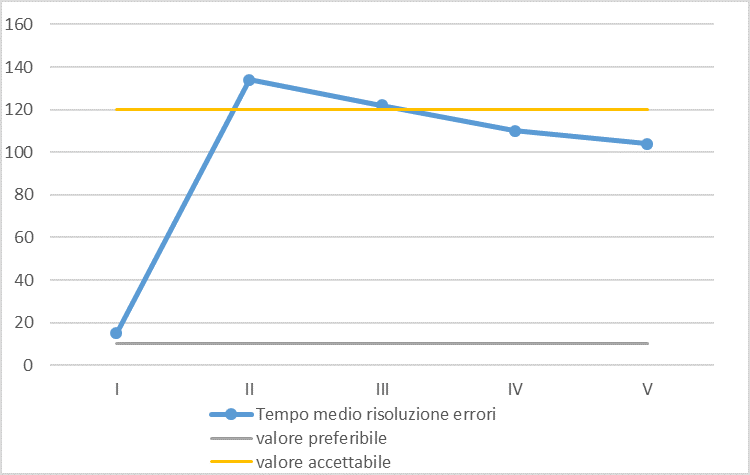
\includegraphics[width=\linewidth]{./img/grafici/RP12.png}	
	\caption{M06 revisione di progettazione\glo}	
\end{figure}
\begin{itemize}
	\item \textbf{Valore preferibile}: $\le10minuti$;
	\item \textbf{Valore accettabile}: $\le120minuti$;
	\item \textbf{Considerazioni}: la metrica\glosp risulta soddisfatta al termine del periodo di progettazione\glo.
\end{itemize}

\paragraph*{PRC-Q5 Processo di gestione organizzativa}
\subparagraph{M07 Planned value} \mbox{}
\begin{longtable}[H!] {						
		>{}p{38mm}  		
		>{}p{12mm}
		>{}p{12mm}		
		>{}p{12mm}		
		>{}p{12mm}		
		>{}p{12mm}		
		>{}p{12mm}
		>{}p{12mm}
		>{}p{12mm}
		>{}p{12mm}
	}
	\rowcolor{gray!50}
	\textbf{} & \textbf{I} & \textbf{II} & \textbf{III} & \textbf{IV} & \textbf{V} \TBstrut \\ [2mm]
	\textbf{PV} & 800\euro & 1868\euro & 2401\euro & 3068\euro & 3836\euro \TBstrut \\ [2mm]
	\rowcolor{white}
	\caption{M07 revisione di progettazione\glo}
\end{longtable}
\begin{figure}[H] 	
	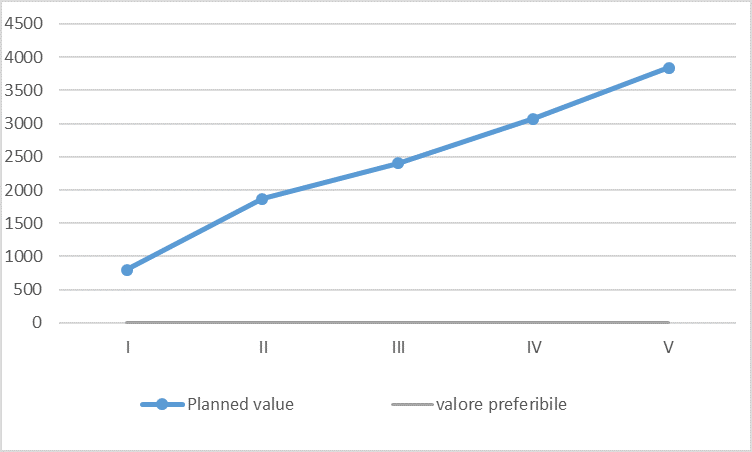
\includegraphics[width=\linewidth]{./img/grafici/RP4.png}	
	\caption{M07 revisione di progettazione\glo}	
\end{figure}
\begin{itemize}
	\item \textbf{Valore preferibile}: $\ge0$;
	\item \textbf{Valore accettabile}: $\ge0$;
	\item \textbf{Considerazioni}: la metrica\glosp risulta soddisfatta al termine del periodo di progettazione\glo.
\end{itemize}
\subparagraph{M08 Earned value} \mbox{}
\begin{longtable}[H!] {						
		>{}p{38mm}  		
		>{}p{12mm}
		>{}p{12mm}		
		>{}p{12mm}		
		>{}p{12mm}		
		>{}p{12mm}		
		>{}p{12mm}
		>{}p{12mm}
		>{}p{12mm}
		>{}p{12mm}
	}
	\rowcolor{gray!50}
	\textbf{} & \textbf{I} & \textbf{II} & \textbf{III} & \textbf{IV} & \textbf{V} \TBstrut \\ [2mm]
	\textbf{EV} & 650\euro & 1300\euro & 2380\euro & 3050\euro & 3836\euro \TBstrut \\ [2mm]
	\rowcolor{white}
	\caption{M08 revisione di progettazione\glo}
\end{longtable}
\begin{figure}[H] 	
	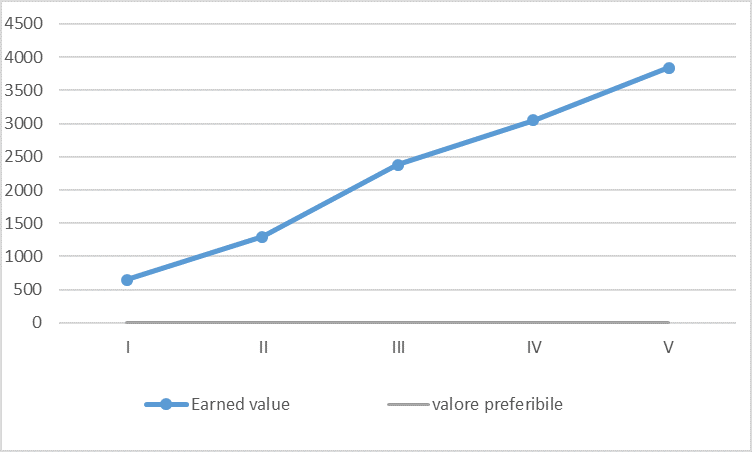
\includegraphics[width=\linewidth]{./img/grafici/RP5.png}	
	\caption{M08 revisione di progettazione\glo}	
\end{figure}
\begin{itemize}
	\item \textbf{Valore preferibile}: $\ge0$;
	\item \textbf{Valore accettabile}: $\ge0$;
	\item \textbf{Considerazioni}: la metrica\glosp risulta soddisfatta al termine del periodo di progettazione\glo.
\end{itemize}
\subparagraph{M09 Actual cost} \mbox{}
\begin{longtable}[H!] {						
		>{}p{38mm}  		
		>{}p{12mm}
		>{}p{12mm}		
		>{}p{12mm}		
		>{}p{12mm}		
		>{}p{12mm}		
		>{}p{12mm}
		>{}p{12mm}
		>{}p{12mm}
		>{}p{12mm}
	}
	\rowcolor{gray!50}
	\textbf{} & \textbf{I} & \textbf{II} & \textbf{III} & \textbf{IV} & \textbf{V} \TBstrut \\ [2mm]
	\textbf{AC} & 1021\euro & 1982\euro & 2582\euro & 3086\euro & 3836\euro \TBstrut \\ [2mm]
	\rowcolor{white}
	\caption{M09 revisione di progettazione\glo}
\end{longtable}
\begin{figure}[H] 	
	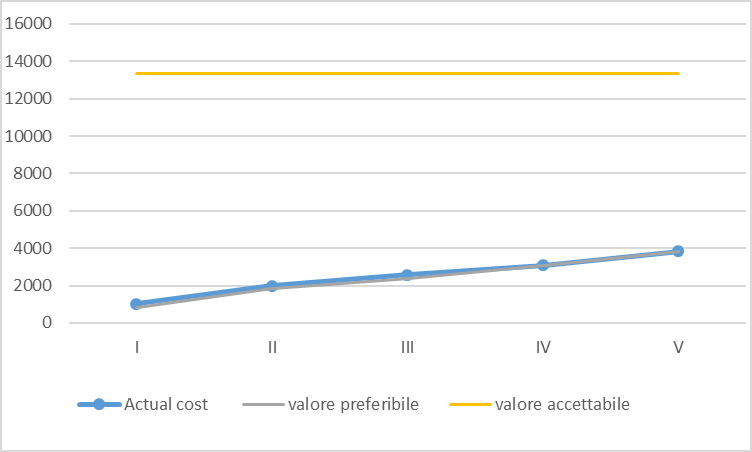
\includegraphics[width=\linewidth]{./img/grafici/RP6.png}	
	\caption{M09 revisione di progettazione\glo}	
	\begin{itemize}
		\item \textbf{Valore preferibile}: $0\le AC \le PV$;
		\item \textbf{Valore accettabile}: $0 \le AC \le budget \; totale$;
		\item \textbf{Considerazioni}: la metrica\glosp risulta soddisfatta al termine del periodo di progettazione\glo.
	\end{itemize}
\end{figure}
\subparagraph{M10 Cost performance index} \mbox{}
\begin{longtable}[H!] {						
		>{}p{50mm}  		
		>{}p{8mm}
		>{}p{8mm}		
		>{}p{8mm}		
		>{}p{8mm}		
		>{}p{8mm}		
		>{}p{8mm}
		>{}p{8mm}
		>{}p{8mm}
		>{}p{8mm}
	}
	\rowcolor{gray!50}
	\textbf{} & \textbf{I} & \textbf{II} & \textbf{III} & \textbf{IV} & \textbf{V} \TBstrut \\ [2mm]
	\textbf{CPI} & 0,64 & 0,66 & 0,92 & 0,99 & 1 \TBstrut \\ [2mm]
	\rowcolor{white}
	\caption{M10 revisione di progettazione\glo}
\end{longtable}
\begin{figure}[H] 	
	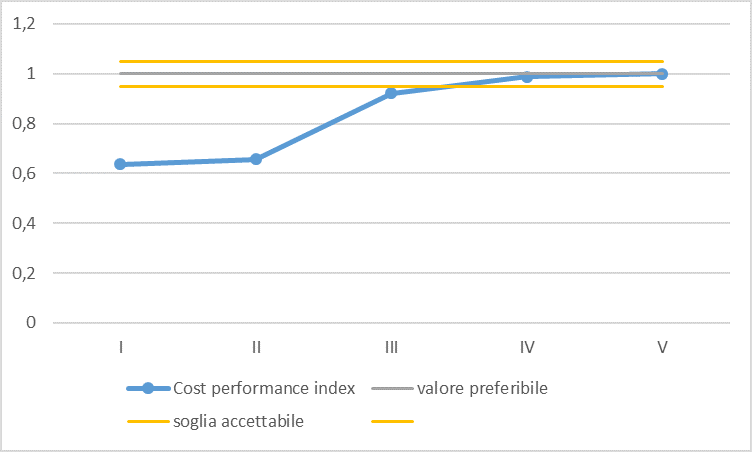
\includegraphics[width=\linewidth]{./img/grafici/RP7.png}	
	\caption{M10 revisione di progettazione\glo}	
\end{figure}
\begin{itemize}
	\item \textbf{Valore preferibile}: $=1$;
	\item \textbf{Valore accettabile}: $0.95 \le CPI \le 1.05$;
	\item \textbf{Considerazioni}: la metrica\glosp risulta soddisfatta al termine del periodo di progettazione\glo.
\end{itemize}
\subparagraph{M11 Schedule performance index} \mbox{}
\begin{longtable}[H!] {						
		>{}p{50mm}  		
		>{}p{8mm}
		>{}p{8mm}		
		>{}p{8mm}		
		>{}p{8mm}		
		>{}p{8mm}		
		>{}p{8mm}
		>{}p{8mm}
		>{}p{8mm}
		>{}p{8mm}
	}
	\rowcolor{gray!50}
	\textbf{} & \textbf{I} & \textbf{II} & \textbf{III} & \textbf{IV} & \textbf{V} \TBstrut \\ [2mm]
	\textbf{SPI} & 0,81 & 0,69 & 0,99 & 0,99 & 1 \TBstrut \\ [2mm]
	\rowcolor{white}
	\caption{M11 revisione di progettazione\glo}
\end{longtable}
\begin{figure}[H] 	
	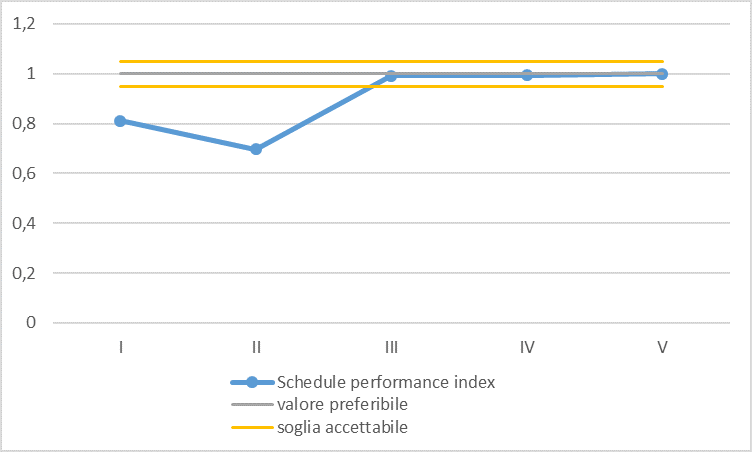
\includegraphics[width=\linewidth]{./img/grafici/RP8.png}	
	\caption{M11 revisione di progettazione\glo}	
\end{figure}
\begin{itemize}
	\item \textbf{Valore preferibile}: $=1$;
	\item \textbf{Valore accettabile}: $0.95 \le SPI \le 1.05$;
	\item \textbf{Considerazioni}: la metrica\glosp risulta soddisfatta al termine del periodo di progettazione\glo.
\end{itemize}
\subparagraph{M12 Estimated cost at compltion} \mbox{}
\begin{longtable}[H!] {						
		>{}p{38mm}  		
		>{}p{12mm}
		>{}p{12mm}		
		>{}p{12mm}		
		>{}p{12mm}		
		>{}p{12mm}		
		>{}p{12mm}
		>{}p{12mm}
		>{}p{12mm}
		>{}p{12mm}
	}
	\rowcolor{gray!50}
	\textbf{} & \textbf{I} & \textbf{II} & \textbf{III} & \textbf{IV} & \textbf{V} \TBstrut \\ [2mm]
	\textbf{EAC} & 20955\euro & 20340\euro & 14473\euro & 13498\euro & 13341\euro \TBstrut \\ [2mm]
	\rowcolor{white}
	\caption{M12 revisione di progettazione\glo}
\end{longtable}
\begin{figure}[H] 	
	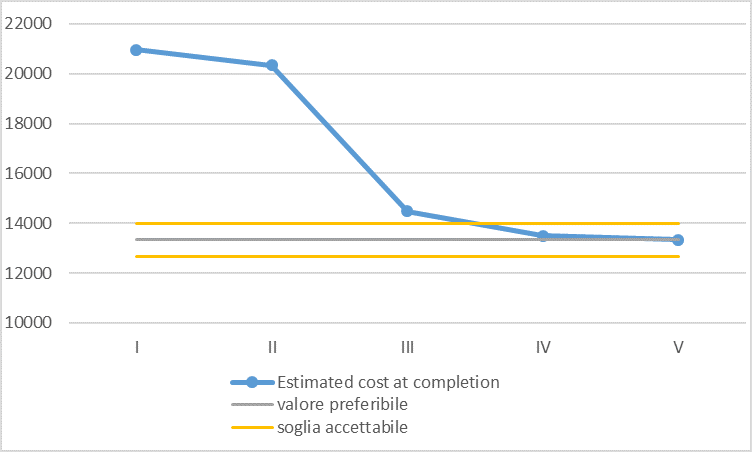
\includegraphics[width=\linewidth]{./img/grafici/RP9.png}	
	\caption{M12 revisione di progettazione\glo}	
\end{figure}
\begin{itemize}
	\item \textbf{Valore preferibile}: pari a quanto preventivato;
	\item \textbf{Valore accettabile}: $preventivo-5\% \le EAC \le preventivo+5\%$;
	\item \textbf{Considerazioni}: la metrica\glosp risulta soddisfatta al termine del periodo di progettazione\glo.
\end{itemize}
\subparagraph{M13 Schedule at completion} \mbox{}
\begin{longtable}[H!] {						
		>{}p{18mm}  		
		>{}p{16mm}
		>{}p{16mm}		
		>{}p{16mm}		
		>{}p{16mm}		
		>{}p{16mm}		
		>{}p{16mm}
		>{}p{16mm}
		>{}p{16mm}
		>{}p{16mm}
	}
	\rowcolor{gray!50}
	\textbf{} & \textbf{I} & \textbf{II} & \textbf{III} & \textbf{IV} & \textbf{V} \TBstrut \\ [2mm]
	\textbf{SAC} & 879 ore & 1026 ore & 720 ore & 718 ore & 714 ore \TBstrut \\ [2mm]
	\rowcolor{white}
	\caption{M13 revisione di progettazione\glo}
\end{longtable}
\begin{figure}[H] 	
	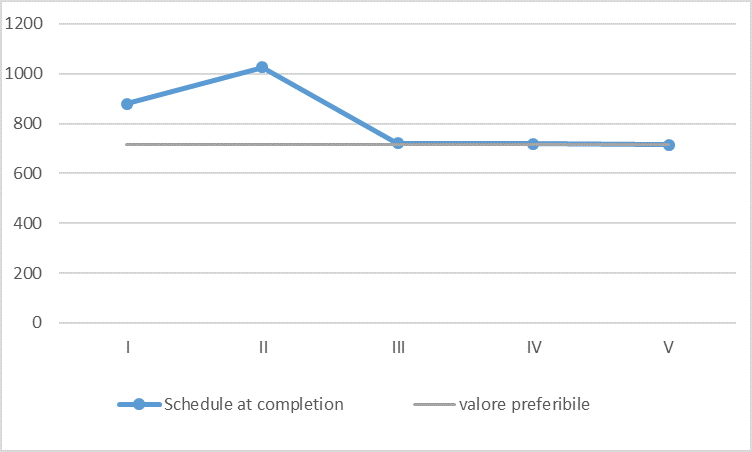
\includegraphics[width=\linewidth]{./img/grafici/RP10.png}	
	\caption{M13 revisione di progettazione\glo}	
\end{figure}
\begin{itemize}
	\item \textbf{Valore preferibile}: pari a quanto preventivato;
	\item \textbf{Valore accettabile}: pari a quanto preventivato;
	\item \textbf{Considerazioni}: la metrica\glosp risulta soddisfatta al termine del periodo di progettazione\glo.
\end{itemize}
\subparagraph{M14 Rischi non preventivati} \mbox{}
\begin{longtable}[H!] {						
		>{}p{50mm}  		
		>{}p{8mm}
		>{}p{8mm}		
		>{}p{8mm}		
		>{}p{8mm}		
		>{}p{8mm}		
		>{}p{8mm}
		>{}p{8mm}
		>{}p{8mm}
		>{}p{8mm}
	}
	\rowcolor{gray!50}
	\textbf{} & \textbf{I} & \textbf{II} & \textbf{III} & \textbf{IV} & \textbf{V} \TBstrut \\ [2mm]
	\textbf{Rischi} & 0 & 0 & 0 & 0 & 0 \TBstrut \\ [2mm]
	\rowcolor{white}
	\caption{M14 revisione di progettazione\glo}
\end{longtable}
\begin{figure}[H] 	
	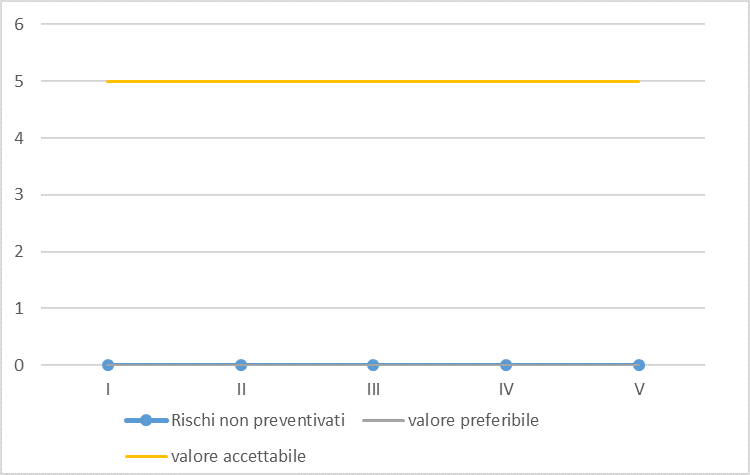
\includegraphics[width=\linewidth]{./img/grafici/RP11.png}	
	\caption{M14 revisione di progettazione\glo}	
\end{figure}
\begin{itemize}
	\item \textbf{Valore preferibile}: $=0$;
	\item \textbf{Valore accettabile}: $\le 5$;
	\item \textbf{Considerazioni}: la metrica\glosp risulta soddisfatta al termine del periodo di progettazione\glo.
\end{itemize}

\paragraph{Qualità di prodotto}
\paragraph*{PRD-Q1 Documenti}
\subparagraph{M15 Indice di Gulpease}\mbox{}
\begin{longtable} {						
		>{}p{50mm}  		
		>{}p{8mm}		
		>{}p{8mm}		
		>{}p{8mm}		
		>{}p{8mm}		
		>{}p{8mm}		
		>{}p{8mm}
		>{}p{8mm}
		>{}p{8mm}
		>{}p{8mm}				
	}			
	\rowcolor{gray!50}
	\textbf{Documento} & \textbf{I} & \textbf{II} & \textbf{III} & \textbf{IV} & \textbf{V} \TBstrut \\ [2mm]
	\textbf{Analisi dei Requisiti} & 93 & 100 & 100 & 100 & 100 \TBstrut \\ [2mm]
	\textbf{Norme di Progetto} & 73 & 79 & 79 & 79 & 81 \TBstrut \\ [2mm]
	\textbf{Piano di Progetto} & 82 & 92 & 75 & 94 & 97 \TBstrut \\ [2mm]
	\textbf{Piano di Qualifica} & 89 & 91 & 87 & 92 & 95 \TBstrut \\ [2mm]
	\textbf{Glossario} & 58 & 83 & 83 & 83 & 83 \TBstrut \\ [2mm]
	\textbf{Verbali interni (media)} & - & 100 & 100 & 100 & 100 \TBstrut \\ [2mm]
	\textbf{Verbali esterni (media)} & - & - & 97 & 97 & 98 \TBstrut \\ [2mm]
	\rowcolor{white}
	\caption{M15 revisione dei requisiti}
\end{longtable}
\begin{figure}[H] 	
	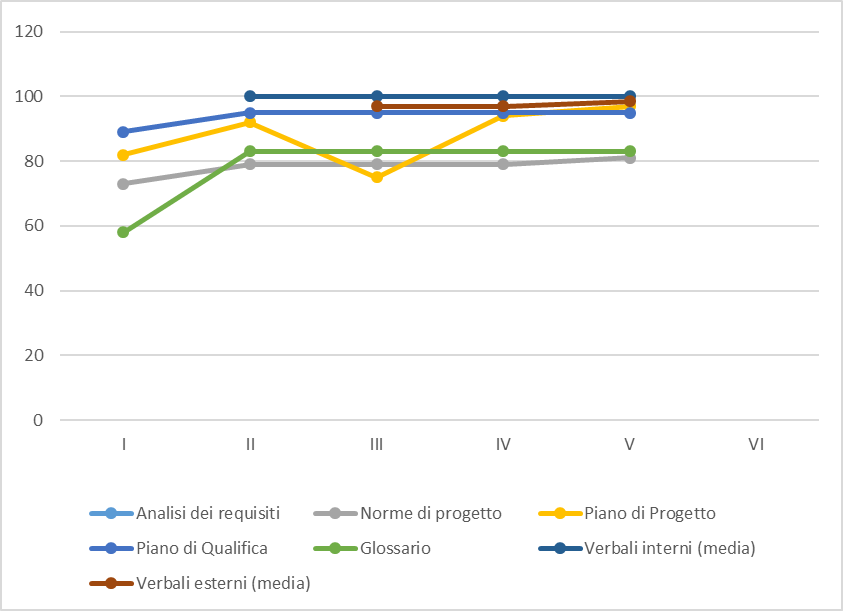
\includegraphics[width=\linewidth]{./img/grafici/RP18.png}	
	\caption{M15 revisione di progettazione}	
\end{figure}
\begin{longtable} {						
		>{}p{70mm}  		
		>{}p{8mm}		
		>{}p{8mm}		
		>{}p{8mm}		
		>{}p{8mm}		
		>{}p{8mm}		
		>{}p{8mm}
		>{}p{8mm}
		>{}p{8mm}
		>{}p{8mm}				
	}			
	\rowcolor{gray!50}
	\textbf{} & \textbf{I} & \textbf{II} & \textbf{III} & \textbf{IV} & \textbf{V} \TBstrut \\ [2mm]
	\textbf{Media dell'indice di Gulpease} & 79 & 90 & 89 & 92 & 93 \TBstrut \\ [2mm]
	\rowcolor{white}
	\caption{M15 revisione dei requisiti}
\end{longtable}
\begin{figure}[H] 	
	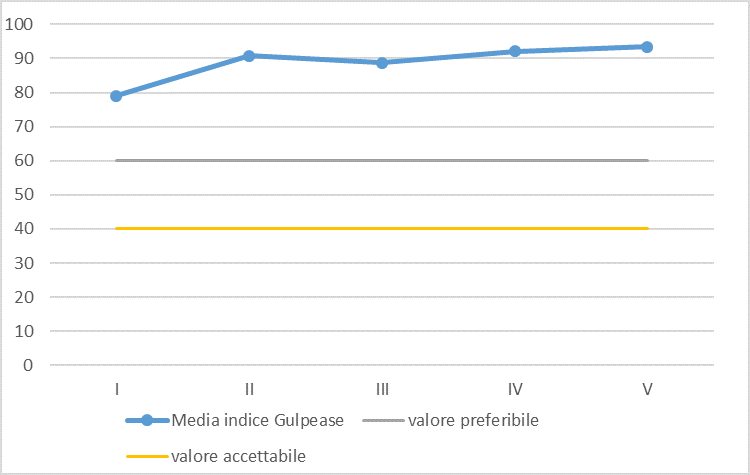
\includegraphics[width=\linewidth]{./img/grafici/RP20.png}	
	\caption{M15 revisione di progettazione}	
\end{figure}
\begin{itemize}
	\item \textbf{Valore preferibile}: $\ge60$;
	\item \textbf{Valore accettabile}: $\ge40$;
	\item \textbf{Considerazioni}: la metrica\glosp risulta soddisfatta al termine del periodo di progettazione\glo.
\end{itemize}
\subparagraph{M19 Correttezza ortografica} \mbox{}
\begin{longtable}[H!] {						
		>{}p{50mm}  		
		>{}p{8mm}
		>{}p{8mm}		
		>{}p{8mm}		
		>{}p{8mm}		
		>{}p{8mm}		
		>{}p{8mm}
		>{}p{8mm}
		>{}p{8mm}
		>{}p{8mm}
	}
	\rowcolor{gray!50}
	\textbf{} & \textbf{I} & \textbf{II} & \textbf{III} & \textbf{IV} & \textbf{V} \TBstrut \\ [2mm]
	\textbf{Numero di metodi} & 0 & 1 & 0 & 0 & 0 \TBstrut \\ [2mm]
	\rowcolor{white}
	\caption{M19 revisione di progettazione\glo}
\end{longtable}
\begin{figure}[H] 	
	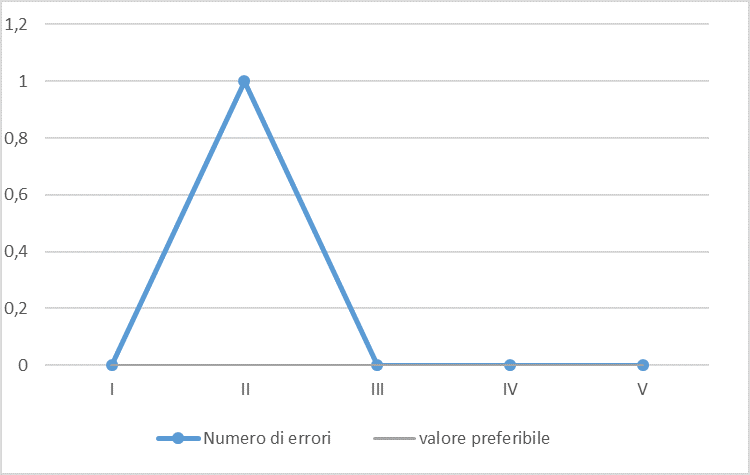
\includegraphics[width=\linewidth]{./img/grafici/RP17.png}	
	\caption{M19 revisione di progettazione\glo}	
\end{figure}
\begin{itemize}
	\item \textbf{Valore preferibile}: $=0$;
	\item \textbf{Valore accettabile}: $=0$;
	\item \textbf{Considerazioni}: la metrica\glosp risulta soddisfatta al termine del periodo di progettazione\glo.
\end{itemize}
\paragraph*{PRD-Q2 Appropriatezza funzionale}
\subparagraph{M16 Percentuale di requisiti obbligatori soddisfatti} \mbox{}
\begin{longtable}[H!] {						
		>{}p{50mm}  		
		>{}p{8mm}
		>{}p{8mm}		
		>{}p{8mm}		
		>{}p{8mm}		
		>{}p{8mm}		
		>{}p{8mm}
		>{}p{8mm}
		>{}p{8mm}
		>{}p{8mm}
	}
	\rowcolor{gray!50}
	\textbf{} & \textbf{I} & \textbf{II} & \textbf{III} & \textbf{IV} & \textbf{V} \TBstrut \\ [2mm]
	\textbf{PROS} & - & - & 32\% & 53\% & 53\% \TBstrut \\ [2mm]
	\rowcolor{white}
	\caption{M16 revisione di progettazione\glo}
\end{longtable}
\begin{figure}[H] 	
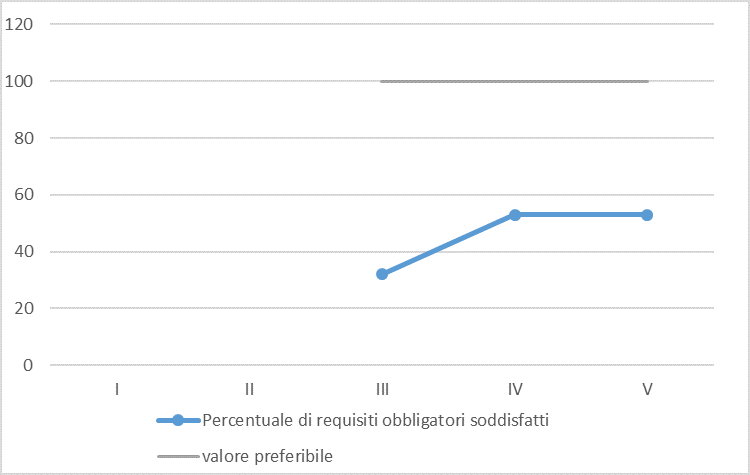
\includegraphics[width=\linewidth]{./img/grafici/RP13.png}	
\caption{M16 revisione di progettazione\glo}	
\end{figure}
\begin{itemize}
	\item \textbf{Valore preferibile}: $=100\%$;
	\item \textbf{Valore accettabile}: $=100\%$;
	\item \textbf{Considerazioni}: la metrica\glosp risulta non soddisfatta al termine del periodo di progettazione\glo.
\end{itemize}
\subparagraph{M17 Percentuale di requisiti desiderabili soddisfatti} \mbox{}
\begin{longtable}[H!] {						
		>{}p{50mm}  		
		>{}p{8mm}
		>{}p{8mm}		
		>{}p{8mm}		
		>{}p{8mm}		
		>{}p{8mm}		
		>{}p{8mm}
		>{}p{8mm}
		>{}p{8mm}
		>{}p{8mm}
	}
	\rowcolor{gray!50}
	\textbf{} & \textbf{I} & \textbf{II} & \textbf{III} & \textbf{IV} & \textbf{V} \TBstrut \\ [2mm]
	\textbf{PRDS} & - & - & 0\% & 0\% & 0\% \TBstrut \\ [2mm]
	\rowcolor{white}
	\caption{M17 revisione di progettazione\glo}
\end{longtable}
\begin{figure}[H] 	
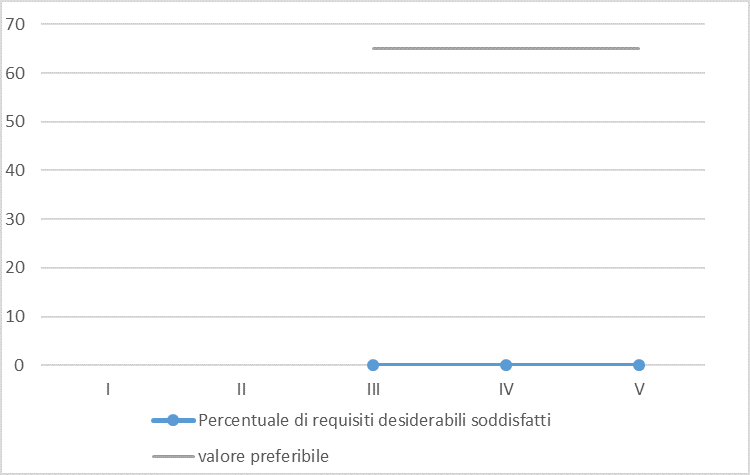
\includegraphics[width=\linewidth]{./img/grafici/RP14.png}	
\caption{M17 revisione di progettazione\glo}	
\end{figure}
\begin{itemize}
	\item \textbf{Valore preferibile}: $\ge 65\%$;
	\item \textbf{Valore accettabile}: $\ge 0\%$;
	\item \textbf{Considerazioni}: la metrica\glosp risulta soddisfatta al termine del periodo di progettazione\glo.
\end{itemize}
\subparagraph{M18 Percentuale di requisiti opzionali soddisfatti} \mbox{}
\begin{longtable}[H!] {						
		>{}p{50mm}  		
		>{}p{8mm}
		>{}p{8mm}		
		>{}p{8mm}		
		>{}p{8mm}		
		>{}p{8mm}		
		>{}p{8mm}
		>{}p{8mm}
		>{}p{8mm}
		>{}p{8mm}
	}
	\rowcolor{gray!50}
	\textbf{} & \textbf{I} & \textbf{II} & \textbf{III} & \textbf{IV} & \textbf{V} \TBstrut \\ [2mm]
	\textbf{PROpS} & - & - & 0\% & 0\% & 0\% \TBstrut \\ [2mm]
	\rowcolor{white}
	\caption{M18 revisione di progettazione\glo}
\end{longtable}
\begin{figure}[H] 	
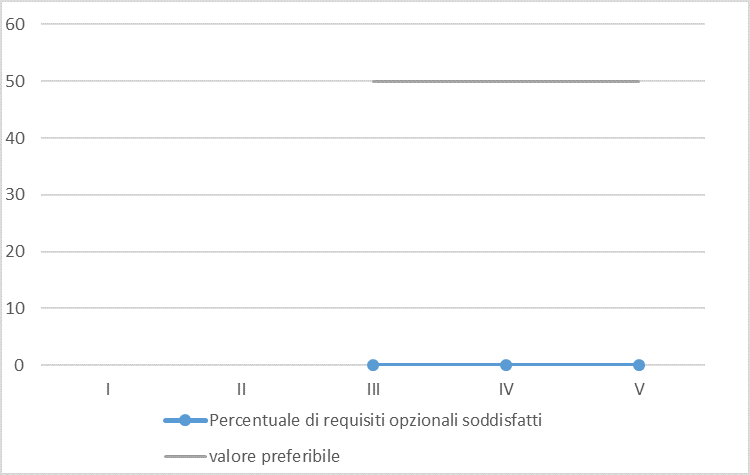
\includegraphics[width=\linewidth]{./img/grafici/RP15.png}	
\caption{M18 revisione di progettazione\glo}	
\end{figure}
\begin{itemize}
	\item \textbf{Valore preferibile}: $\ge50\%$;
	\item \textbf{Valore accettabile}: $\ge0\%$;
	\item \textbf{Considerazioni}: la metrica\glosp risulta soddisfatta al termine del periodo di progettazione\glo.
\end{itemize}

\subsubsection{Revisioni generali}\mbox{}
\begin{longtable} {						
		>{}p{50mm}  		
		>{}p{8mm}		
		>{}p{8mm}		
		>{}p{8mm}		
		>{}p{8mm}		
		>{}p{8mm}		
		>{}p{8mm}
		>{}p{8mm}				
	}			
	\rowcolor{gray!50}
	\textbf{Metrica} & \textbf{RR} & \textbf{RP} & \textbf{RQ} & \textbf{RA} \TBstrut \\ [2mm]
	\textbf{M01} & - & 29 & - & - \TBstrut \\ [2mm]
	\textbf{M02} & - & 4 & - & - \TBstrut \\ [2mm]
	\textbf{M03} & - & 21 & - & - \TBstrut \\ [2mm]
	\textbf{M15} & 82 & 93 & - & - \TBstrut \\ [2mm]
	\textbf{M19} & - & 0 & - & - \TBstrut \\ [2mm]
	\textbf{M07} & - & 3836 & - & - \TBstrut \\ [2mm]
	\textbf{M08} & - & 3836 & - & - \TBstrut \\ [2mm]
	\textbf{M09} & - & 3836 & - & - \TBstrut \\ [2mm]
	\textbf{M10} & - & 1 & - & - \TBstrut \\ [2mm]
	\textbf{M11} & - & 1 & - & - \TBstrut \\ [2mm]
	\textbf{M12} & - & 13341 & - & - \TBstrut \\ [2mm]
	\textbf{M13} & - & 714 & - & - \TBstrut \\ [2mm]
	\textbf{M14} & - & 0 & - & - \TBstrut \\ [2mm]
	\textbf{M06} & - & 104 & - & - \TBstrut \\ [2mm]
	\textbf{M16} & - & 53 & - & - \TBstrut \\ [2mm]
	\textbf{M17} & - & 0 & - & - \TBstrut \\ [2mm]
	\textbf{M18} & - & 0 & - & - \TBstrut \\ [2mm]
	\textbf{M05} & - & 40 & - & - \TBstrut \\ [2mm]
	\textbf{M04} & - & 78 & - & - \TBstrut \\ [2mm]
	\rowcolor{white}
	\caption{Revisione generale}
\end{longtable}




\subsection{Revisione di qualifica (RQ)}
\subsubsection{Riassunto delle attività di verifica}
In questo periodo abbiamo attuato le verifiche sui documenti, sulla codifica e sulla pianificazione come nel precedente periodo. A queste abbiamo aggiunto le verifiche sulla progettazione e sui testi per verificare che lo svolgimento del progetto\glosp procedesse senza impedimenti.  
\paragraph{Analisi statica dei documenti}
L'analisi statica\glosp dei documenti ha portato alla produzione di una lista degli errori comuni ridotti rispetto alla revisione precedente. Questa lista deve essere aggiornata con le prossime analisi e andrà a facilitare il compito dei verificatori.
\subsubsection{Esiti delle verifiche} 
\paragraph{Qualità di processo}
\paragraph*{PRC-Q1 Processo di sviluppo}
\subparagraph{M01 Scostamento dei requisiti individuati} \mbox{}
\begin{longtable}[H!] {						
		>{}p{50mm}  		
		>{}p{8mm}
		>{}p{8mm}		
		>{}p{8mm}		
		>{}p{8mm}		
		>{}p{8mm}		
		>{}p{8mm}
		>{}p{8mm}
		>{}p{8mm}
		>{}p{8mm}
	}
	\rowcolor{gray!50}
	\textbf{} & \textbf{I} & \textbf{II} & \textbf{III} & \textbf{IV} & \textbf{V} & \textbf{VI} \TBstrut \\ [2mm]
	\textbf{Scostamenti} & 1 & 0 & 0 & 0 & 0 & 0 \TBstrut \\ [2mm]
	\rowcolor{white}
	\caption{M01 revisione di qualifica}
\end{longtable}
\begin{figure}[H] 	
	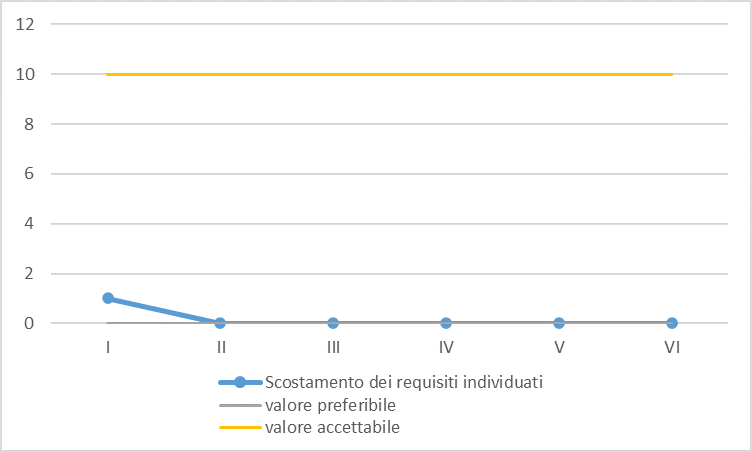
\includegraphics[width=\linewidth]{./img/grafici/RQ1.png}	
	\caption{M01 revisione di qualifica}	
\end{figure}
\begin{itemize}
	\item \textbf{Valore preferibile}: 0;
	\item \textbf{Valore accettabile}: 10;
	\item \textbf{Considerazioni}: la metrica\glosp risulta soddisfatta al termine del periodo di qualifica.
\end{itemize}

\subparagraph{M02 Numero di parametri per metodo} \mbox{}
\begin{longtable}[H!] {						
		>{}p{50mm}  		
		>{}p{8mm}
		>{}p{8mm}		
		>{}p{8mm}		
		>{}p{8mm}		
		>{}p{8mm}		
		>{}p{8mm}
		>{}p{8mm}
		>{}p{8mm}
		>{}p{8mm}
	}
	\rowcolor{gray!50}
	\textbf{} & \textbf{I} & \textbf{II} & \textbf{III} & \textbf{IV} & \textbf{V} & \textbf{VI} \TBstrut \\ [2mm]
	\textbf{Numero} & 4 & 5 & 5 & 5 & 5 & 5 \TBstrut \\ [2mm]
	\rowcolor{white}
	\caption{M02 revisione di qualifica}
\end{longtable}
\begin{figure}[H] 	
	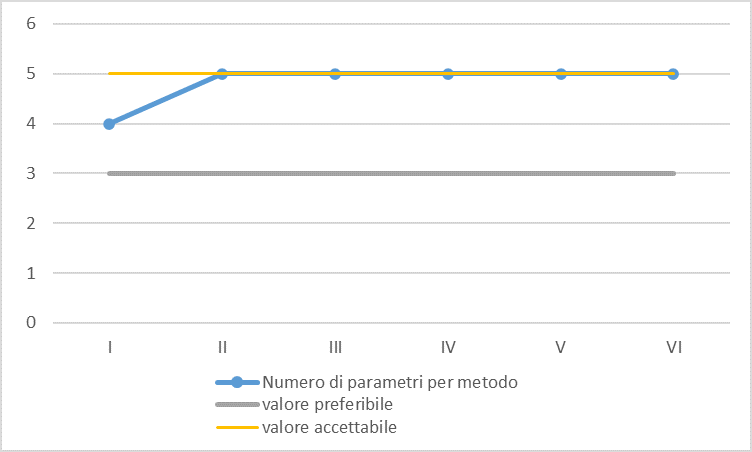
\includegraphics[width=\linewidth]{./img/grafici/RQ2.png}	
	\caption{M02 revisione di qualifica}	
\end{figure}
\begin{itemize}
	\item \textbf{Valore preferibile}: $\le 3$;
	\item \textbf{Valore accettabile}: $\le 5$;
	\item \textbf{Considerazioni}: la metrica\glosp risulta soddisfatta al termine del periodo di qualifica.
\end{itemize}

\subparagraph{M03 Numero di metodi per classe} \mbox{}
\begin{longtable}[H!] {						
		>{}p{50mm}  		
		>{}p{8mm}
		>{}p{8mm}		
		>{}p{8mm}		
		>{}p{8mm}		
		>{}p{8mm}		
		>{}p{8mm}
		>{}p{8mm}
		>{}p{8mm}
		>{}p{8mm}
	}
	\rowcolor{gray!50}
	\textbf{} & \textbf{I} & \textbf{II} & \textbf{III} & \textbf{IV} & \textbf{V} & \textbf{VI} \TBstrut \\ [2mm]
	\textbf{Numero} & 15 & 15 & 15 & 14 & 16 & 15 \TBstrut \\ [2mm]
	\rowcolor{white}
	\caption{M03 revisione di qualifica}
\end{longtable}
\begin{figure}[H] 	
	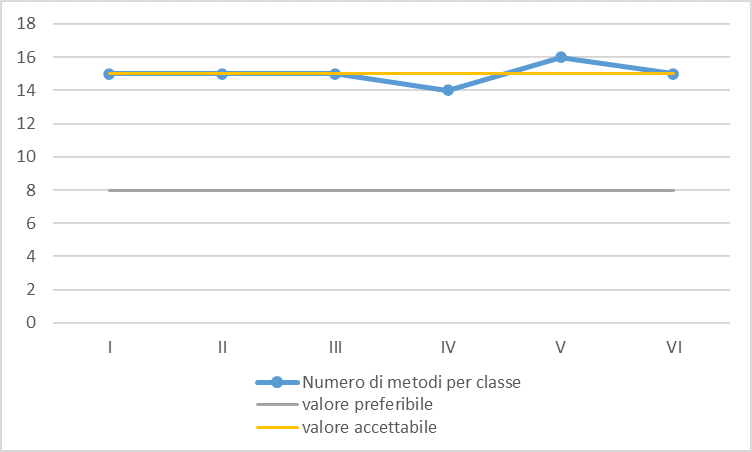
\includegraphics[width=\linewidth]{./img/grafici/RQ3.png}	
	\caption{M03 revisione di qualifica}	
\end{figure}
\begin{itemize}
	\item \textbf{Valore preferibile}: $\le 8$;
	\item \textbf{Valore accettabile}: $\le 15$;
	\item \textbf{Considerazioni}: la metrica\glosp risulta soddisfatta al termine del periodo di qualifica.
\end{itemize}

\subparagraph{M20 Livello di annidamento} \mbox{}
\begin{longtable}[H!] {						
		>{}p{50mm}  		
		>{}p{8mm}
		>{}p{8mm}		
		>{}p{8mm}		
		>{}p{8mm}		
		>{}p{8mm}		
		>{}p{8mm}
		>{}p{8mm}
		>{}p{8mm}
		>{}p{8mm}
	}
	\rowcolor{gray!50}
	\textbf{} & \textbf{I} & \textbf{II} & \textbf{III} & \textbf{IV} & \textbf{V} & \textbf{VI} \TBstrut \\ [2mm]
	\textbf{Livello} & 1 & 1 & 2 & 2 & 2 & 2 \TBstrut \\ [2mm]
	\rowcolor{white}
	\caption{M20 revisione di qualifica}
\end{longtable}
\begin{figure}[H] 	
	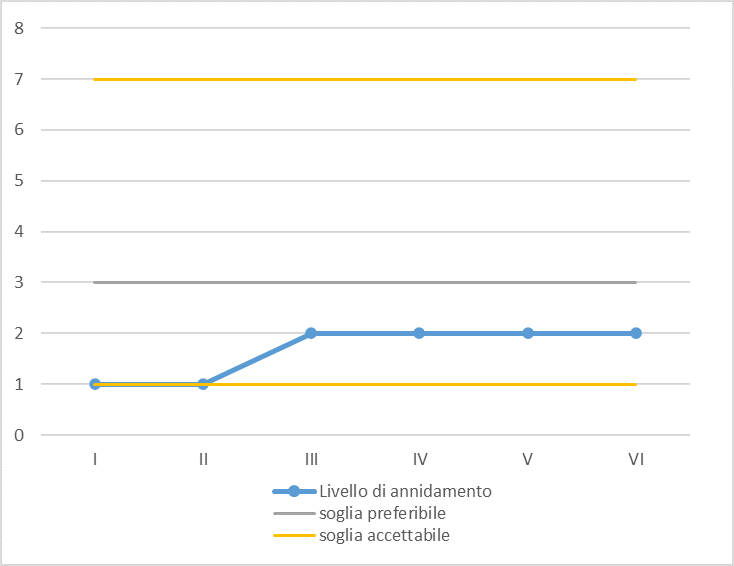
\includegraphics[width=\linewidth]{./img/grafici/RQ20.png}	
	\caption{M20 revisione di qualifica}	
\end{figure}
\begin{itemize}
	\item \textbf{Valore preferibile}: $1\le x \le 3$;
	\item \textbf{Valore accettabile}: $1 \le x \le 7$;
	\item \textbf{Considerazioni}: la metrica\glosp risulta soddisfatta al termine del periodo di qualifica.
\end{itemize}
\paragraph{M21 Profondità gerarchia} \mbox{}
\begin{longtable}[H!] {						
		>{}p{50mm}  		
		>{}p{8mm}
		>{}p{8mm}		
		>{}p{8mm}		
		>{}p{8mm}		
		>{}p{8mm}		
		>{}p{8mm}
		>{}p{8mm}
		>{}p{8mm}
		>{}p{8mm}
	}
	\rowcolor{gray!50}
	\textbf{} & \textbf{I} & \textbf{II} & \textbf{III} & \textbf{IV} & \textbf{V} & \textbf{VI} \TBstrut \\ [2mm]
	\textbf{Profondità} & 2 & 2 & 2 & 2 & 2 & 2 \TBstrut \\ [2mm]
	\rowcolor{white}
	\caption{M21 revisione di qualifica}
\end{longtable}
\begin{figure}[H] 	
	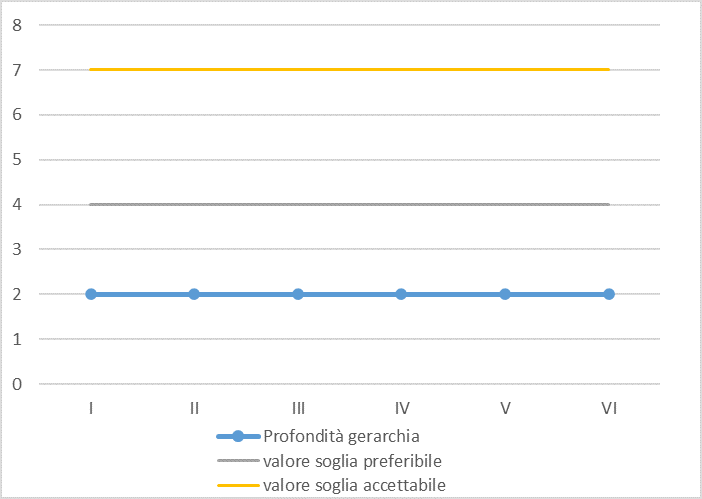
\includegraphics[width=\linewidth]{./img/grafici/RQ21.png}	
	\caption{M21 revisione di qualifica}	
\end{figure}
\begin{itemize}
	\item \textbf{Valore preferibile}: $\le 4$;
	\item \textbf{Valore accettabile}: $\le 7$;
	\item \textbf{Considerazioni}: la metrica\glosp risulta soddisfatta al termine del periodo di qualifica.
\end{itemize}

\paragraph{M22 Numero di design pattern} \mbox{}
\begin{longtable}[H!] {						
		>{}p{50mm}  		
		>{}p{8mm}
		>{}p{8mm}		
		>{}p{8mm}		
		>{}p{8mm}		
		>{}p{8mm}		
		>{}p{8mm}
		>{}p{8mm}
		>{}p{8mm}
		>{}p{8mm}
	}
	\rowcolor{gray!50}
	\textbf{} & \textbf{I} & \textbf{II} & \textbf{III} & \textbf{IV} & \textbf{V} & \textbf{VI} \TBstrut \\ [2mm]
	\textbf{Numero} & 4 & 6 & 6 & 6 & 6 & 6 \TBstrut \\ [2mm]
	\rowcolor{white}
	\caption{M22 revisione di qualifica}
\end{longtable}
\begin{figure}[H] 	
	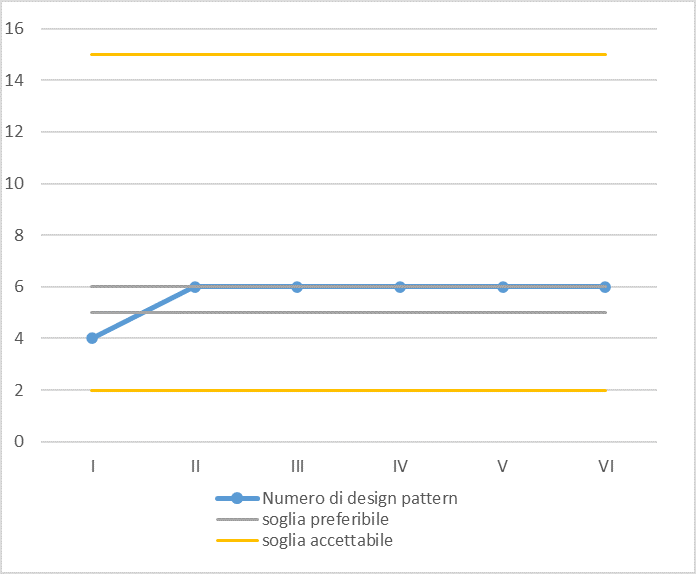
\includegraphics[width=\linewidth]{./img/grafici/RQ22.png}	
	\caption{M22 revisione di qualifica}	
\end{figure}
\begin{itemize}
	\item \textbf{Valore preferibile}: $5\le x \le 6$;
	\item \textbf{Valore accettabile}: $2 \le x \le 15$;
	\item \textbf{Considerazioni}: la metrica\glosp risulta soddisfatta al termine del periodo di qualifica.
\end{itemize}


\paragraph*{PRC-Q3 Processo di verifica}
\subparagraph{M05 Percentuale bug sistemati} \mbox{}
\begin{longtable}[H!] {						
		>{}p{50mm}  		
		>{}p{8mm}
		>{}p{8mm}		
		>{}p{8mm}		
		>{}p{8mm}		
		>{}p{8mm}		
		>{}p{8mm}
		>{}p{8mm}
		>{}p{8mm}
		>{}p{8mm}
	}
	\rowcolor{gray!50}
	\textbf{} & \textbf{I} & \textbf{II} & \textbf{III} & \textbf{IV} & \textbf{V} \TBstrut \\ [2mm]
	\textbf{Percentuale} & 70\% & 80\% & 100\% & 100\% & 100\% \TBstrut \\ [2mm]
	\rowcolor{white}
	\caption{M05 revisione di qualifica}
\end{longtable}
\begin{figure}[H] 	
	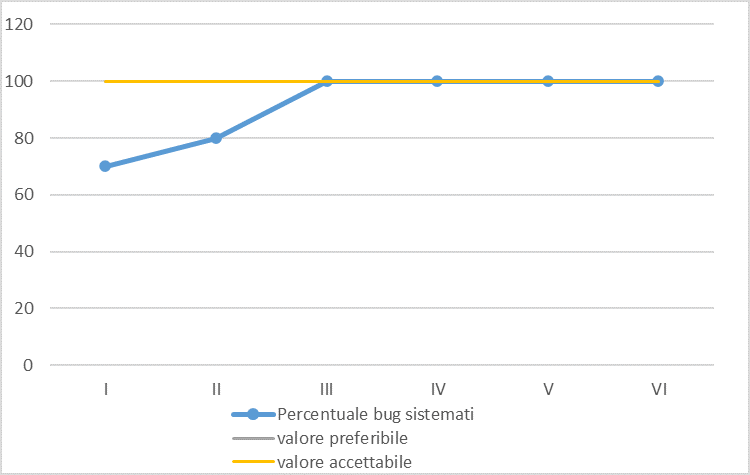
\includegraphics[width=\linewidth]{./img/grafici/RQ5.png}	
	\caption{M05 revisione di qualifica}	
\end{figure}
\begin{itemize}
	\item \textbf{Valore preferibile}: $=100\%$;
	\item \textbf{Valore accettabile}: $=100\%$;
	\item \textbf{Considerazioni}: la metrica\glosp risulta soddisfatta al termine del periodo di qualifica.
\end{itemize}

\paragraph{M25 Copertura test eseguiti} \mbox{}
\begin{longtable}[H!] {						
		>{}p{50mm}  		
		>{}p{8mm}
		>{}p{8mm}		
		>{}p{8mm}		
		>{}p{8mm}		
		>{}p{8mm}		
		>{}p{8mm}
		>{}p{8mm}
		>{}p{8mm}
		>{}p{8mm}
	}
	\rowcolor{gray!50}
	\textbf{} & \textbf{I} & \textbf{II} & \textbf{III} & \textbf{IV} & \textbf{V} & \textbf{VI} \TBstrut \\ [2mm]
	\textbf{Percentuale} & 100\% & 100\% & 100\% & 100\% & 100\% & 100\% \TBstrut \\ [2mm]
	\rowcolor{white}
	\caption{M25 revisione di qualifica}
\end{longtable}
\begin{figure}[H] 	
	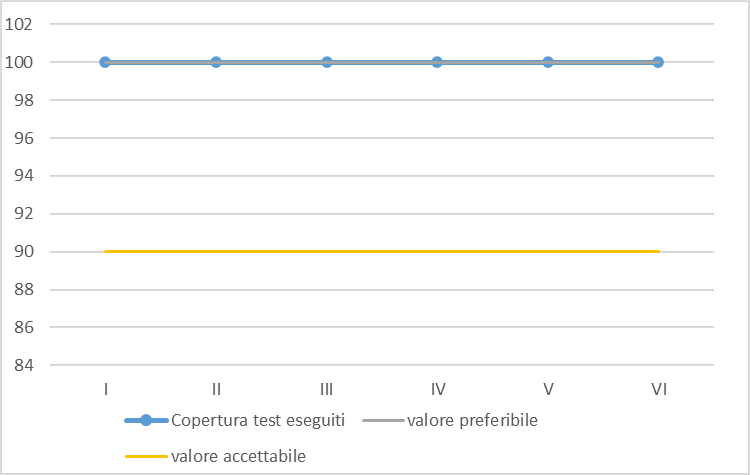
\includegraphics[width=\linewidth]{./img/grafici/RQ25.png}	
	\caption{M25 revisione di qualifica}	
\end{figure}
\begin{itemize}
	\item \textbf{Valore preferibile}: $\ge 90\%$
	\item \textbf{Valore accettabile}: $100\%$
	\item \textbf{Considerazioni}: la metrica\glosp risulta soddisfatta al termine del periodo di qualifica.
\end{itemize}

\paragraph*{PRC-Q4 Processo di gestione dei cambiamenti}
\subparagraph{M06 Tempo medio risoluzione errori} \mbox{}
\begin{longtable}[H!] {						
		>{}p{50mm}  		
		>{}p{8mm}
		>{}p{8mm}		
		>{}p{8mm}		
		>{}p{8mm}		
		>{}p{8mm}		
		>{}p{8mm}
		>{}p{8mm}
		>{}p{8mm}
		>{}p{8mm}
	}
	\rowcolor{gray!50}
	\textbf{} & \textbf{I} & \textbf{II} & \textbf{III} & \textbf{IV} & \textbf{V} & \textbf{VI} \TBstrut \\ [2mm]
	\textbf{Tempo medio} & 20min & 25min & 16min & 40min & 50min & 52min \TBstrut \\ [2mm]
	\rowcolor{white}
	\caption{M06 revisione di qualifica}
\end{longtable}
\begin{figure}[H] 	
	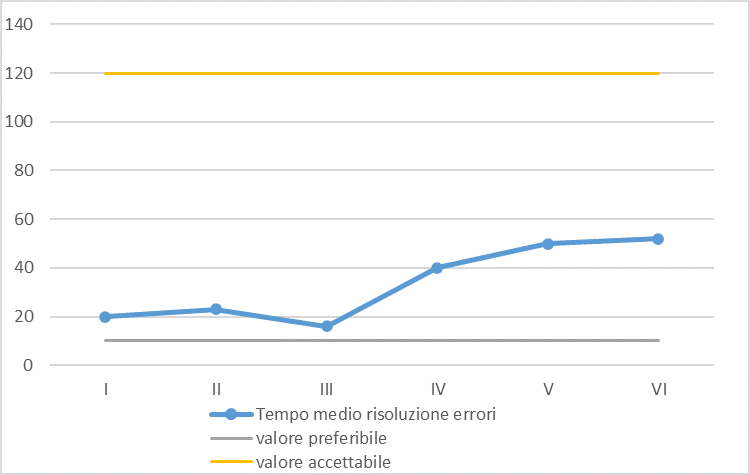
\includegraphics[width=\linewidth]{./img/grafici/RQ6.png}	
	\caption{M06 revisione di qualifica}	
\end{figure}
\begin{itemize}
	\item \textbf{Valore preferibile}: $\le10minuti$;
	\item \textbf{Valore accettabile}: $\le120minuti$;
	\item \textbf{Considerazioni}: la metrica\glosp risulta soddisfatta al termine del periodo di qualifica.
\end{itemize}

\paragraph{PRC-Q5 Processo di gestione organizzativa}
\subparagraph{M07 Planned Value} \mbox{}
\begin{longtable}[H!] {						
		>{}p{50mm}  		
		>{}p{8mm}
		>{}p{8mm}		
		>{}p{8mm}		
		>{}p{8mm}		
		>{}p{8mm}		
		>{}p{8mm}
		>{}p{8mm}
		>{}p{8mm}
		>{}p{8mm}
	}
	\rowcolor{gray!50}
	\textbf{} & \textbf{I} & \textbf{II} & \textbf{III} & \textbf{IV} & \textbf{V} & \textbf{VI} \TBstrut \\ [2mm]
	\textbf{PV} & 2290 & 3830 & 4640 & 5185 & 6635 & 7160 \TBstrut \\ [2mm]
	\rowcolor{white}
	\caption{M07 revisione di qualifica}
\end{longtable}
\begin{figure}[H] 	
	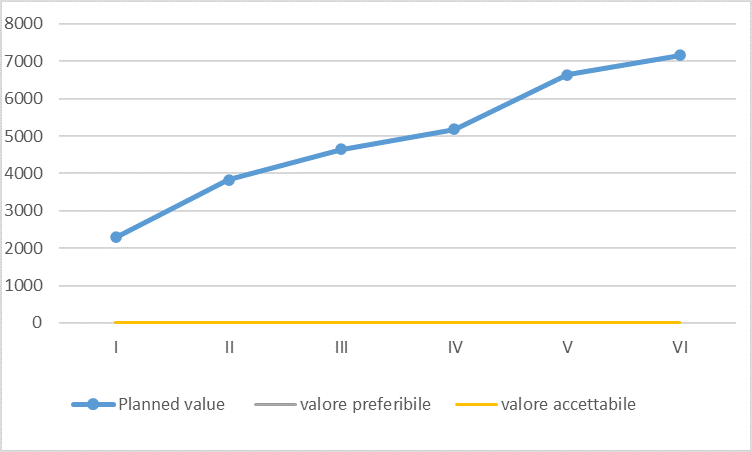
\includegraphics[width=\linewidth]{./img/grafici/RQ7.png}	
	\caption{M07 revisione di qualifica}	
\end{figure}
\begin{itemize}
	\item \textbf{Valore preferibile}: $\ge0$;
	\item \textbf{Valore accettabile}: $\ge0$;
	\item \textbf{Considerazioni}: la metrica\glosp risulta soddisfatta al termine del periodo di qualifica.
\end{itemize}

\subparagraph{M08 Earned Value} \mbox{}
\begin{longtable}[H!] {						
		>{}p{50mm}  		
		>{}p{8mm}
		>{}p{8mm}		
		>{}p{8mm}		
		>{}p{8mm}		
		>{}p{8mm}		
		>{}p{8mm}
		>{}p{8mm}
		>{}p{8mm}
		>{}p{8mm}
	}
	\rowcolor{gray!50}
	\textbf{} & \textbf{I} & \textbf{II} & \textbf{III} & \textbf{IV} & \textbf{V} & \textbf{VI} \TBstrut \\ [2mm]
	\textbf{EV} & 2290 & 3830 & 4640 & 5185 & 6635 & 7160 \TBstrut \\ [2mm]
	\rowcolor{white}
	\caption{M08 revisione di qualifica}
\end{longtable}
\begin{figure}[H] 	
	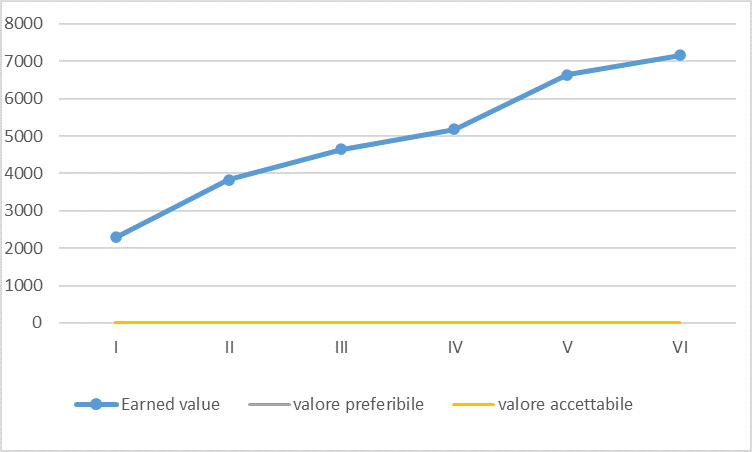
\includegraphics[width=\linewidth]{./img/grafici/RQ8.png}	
	\caption{M08 revisione di qualifica}	
\end{figure}
\begin{itemize}
	\item \textbf{Valore preferibile}: $\ge0$;
	\item \textbf{Valore accettabile}: $\ge0$;
	\item \textbf{Considerazioni}: la metrica\glosp risulta soddisfatta al termine del periodo di qualifica.
\end{itemize}

\subparagraph{M09 Actual Cost} \mbox{}
\begin{longtable}[H!] {						
		>{}p{50mm}  		
		>{}p{8mm}
		>{}p{8mm}		
		>{}p{8mm}		
		>{}p{8mm}		
		>{}p{8mm}		
		>{}p{8mm}
		>{}p{8mm}
		>{}p{8mm}
		>{}p{8mm}
	}
	\rowcolor{gray!50}
	\textbf{} & \textbf{I} & \textbf{II} & \textbf{III} & \textbf{IV} & \textbf{V} & \textbf{VI} \TBstrut \\ [2mm]
	\textbf{AC} & 2282 & 3778 & 4588 & 5155 & 6678 & 7159 \TBstrut \\ [2mm]
	\rowcolor{white}
	\caption{M09 revisione di qualifica}
\end{longtable}
\begin{figure}[H] 	
	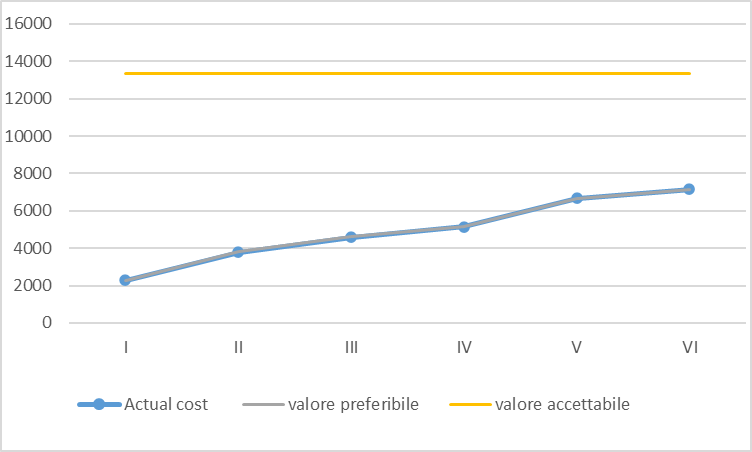
\includegraphics[width=\linewidth]{./img/grafici/RQ9.png}	
	\caption{M09 revisione di qualifica}	
\end{figure}
\begin{itemize}
	\item \textbf{Valore preferibile}: $0\le AC \le PV$;
	\item \textbf{Valore accettabile}: $0 \le AC \le budget \; totale$;
	\item \textbf{Considerazioni}: la metrica\glosp risulta soddisfatta al termine del periodo di qualifica.
\end{itemize}

\subparagraph{M10 Cost perform index} \mbox{}
\begin{longtable}[H!] {						
		>{}p{50mm}  		
		>{}p{8mm}
		>{}p{8mm}		
		>{}p{8mm}		
		>{}p{8mm}		
		>{}p{8mm}		
		>{}p{8mm}
		>{}p{8mm}
		>{}p{8mm}
		>{}p{8mm}
	}
	\rowcolor{gray!50}
	\textbf{} & \textbf{I} & \textbf{II} & \textbf{III} & \textbf{IV} & \textbf{V} & \textbf{VI} \TBstrut \\ [2mm]
	\textbf{CPI} & 1 & 1,01 & 1,01 & 1 & 0,99 & 1 \TBstrut \\ [2mm]
	\rowcolor{white}
	\caption{M10 revisione di qualifica}
\end{longtable}
\begin{figure}[H] 	
	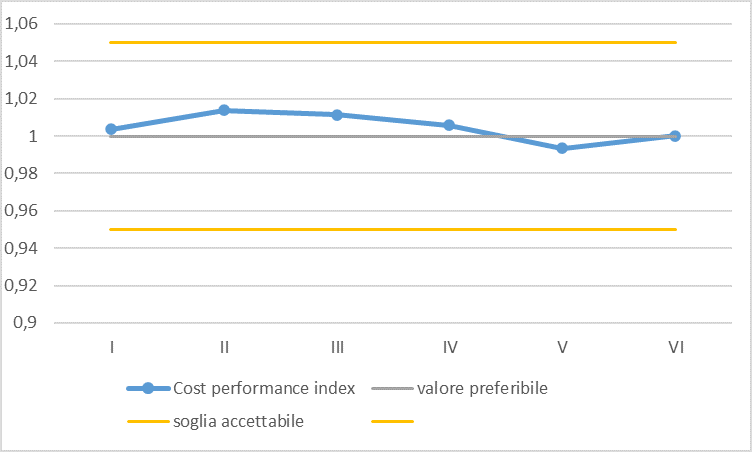
\includegraphics[width=\linewidth]{./img/grafici/RQ10.png}	
	\caption{M10 revisione di qualifica}	
\end{figure}
\begin{itemize}
	\item \textbf{Valore preferibile}: $=1$;
	\item \textbf{Valore accettabile}: $0.95 \le CPI \le 1.05$;
	\item \textbf{Considerazioni}: la metrica\glosp risulta soddisfatta al termine del periodo di qualifica.
\end{itemize}

\subparagraph{M11 Schedule perform index} \mbox{}
\begin{longtable}[H!] {						
		>{}p{50mm}  		
		>{}p{8mm}
		>{}p{8mm}		
		>{}p{8mm}		
		>{}p{8mm}		
		>{}p{8mm}		
		>{}p{8mm}
		>{}p{8mm}
		>{}p{8mm}
		>{}p{8mm}
	}
	\rowcolor{gray!50}
	\textbf{} & \textbf{I} & \textbf{II} & \textbf{III} & \textbf{IV} & \textbf{V} & \textbf{VI} \TBstrut \\ [2mm]
	\textbf{SPI} & 1 & 1 & 1 & 1 & 1 & 1 \TBstrut \\ [2mm]
	\rowcolor{white}
	\caption{M11 revisione di qualifica}
\end{longtable}
\begin{figure}[H] 	
	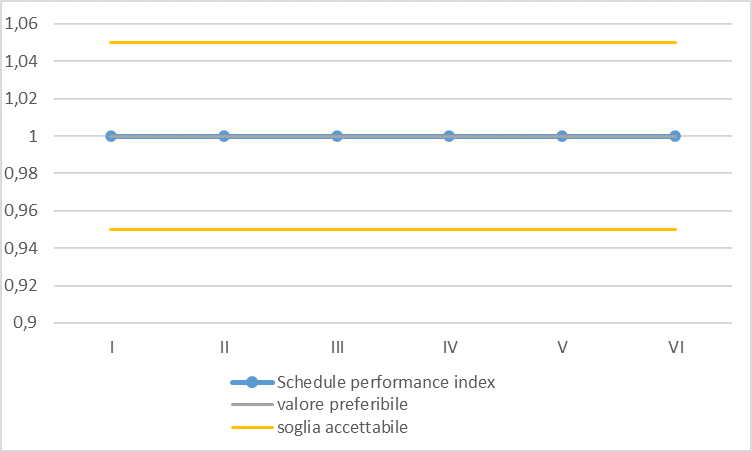
\includegraphics[width=\linewidth]{./img/grafici/RQ11.png}	
	\caption{M11 revisione di qualifica}	
\end{figure}
	\begin{itemize}
		\item \textbf{Valore preferibile}: $=1$;
		\item \textbf{Valore accettabile}: $0.95 \le SPI \le 1.05$;
		\item \textbf{Considerazioni}: la metrica\glosp risulta soddisfatta al termine del periodo di qualifica.
	\end{itemize}

\subparagraph{M12 Estimated cost at completion} \mbox{}
\begin{longtable}[H!] {						
		>{}p{25mm}  		
		>{}p{12mm}
		>{}p{12mm}		
		>{}p{12mm}		
		>{}p{12mm}		
		>{}p{12mm}		
		>{}p{12mm}
		>{}p{12mm}
		>{}p{12mm}
		>{}p{12mm}
	}
	\rowcolor{gray!50}
	\textbf{} & \textbf{I} & \textbf{II} & \textbf{III} & \textbf{IV} & \textbf{V} & \textbf{VI} \TBstrut \\ [2mm]
	\textbf{Costo} & 13333\euro & 13289\euro & 13289\euro & 13311\euro & 13384\euro & 13340\euro \TBstrut \\ [2mm]
	\rowcolor{white}
	\caption{M12 revisione di qualifica}
\end{longtable}
\begin{figure}[H] 	
	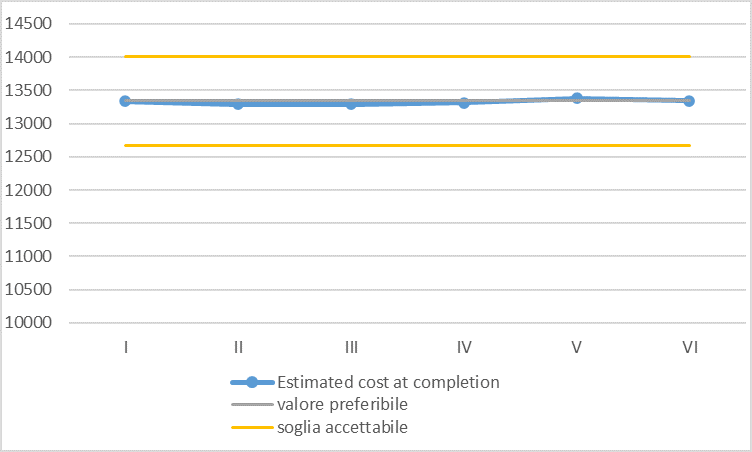
\includegraphics[width=\linewidth]{./img/grafici/RQ12.png}	
	\caption{M12 revisione di qualifica}	
\end{figure}
\begin{itemize}
	\item \textbf{Valore preferibile}: pari a quanto preventivato;
	\item \textbf{Valore accettabile}: $preventivo-5\% \le EAC \le preventivo+5\%$;
	\item \textbf{Considerazioni}: la metrica\glosp risulta soddisfatta al termine del periodo di qualifica.
\end{itemize}


\subparagraph{M13 Schedule at completion} \mbox{}
\begin{longtable}[H!] {						
		>{}p{50mm}  		
		>{}p{8mm}
		>{}p{8mm}		
		>{}p{8mm}		
		>{}p{8mm}		
		>{}p{8mm}		
		>{}p{8mm}
		>{}p{8mm}
		>{}p{8mm}
		>{}p{8mm}
	}
	\rowcolor{gray!50}
	\textbf{} & \textbf{I} & \textbf{II} & \textbf{III} & \textbf{IV} & \textbf{V} & \textbf{VI} \TBstrut \\ [2mm]
	\textbf{Ore} & 714 & 714 & 714 & 714 & 714 & 714 \TBstrut \\ [2mm]
	\rowcolor{white}
	\caption{M13 revisione di qualifica}
\end{longtable}
\begin{figure}[H] 	
	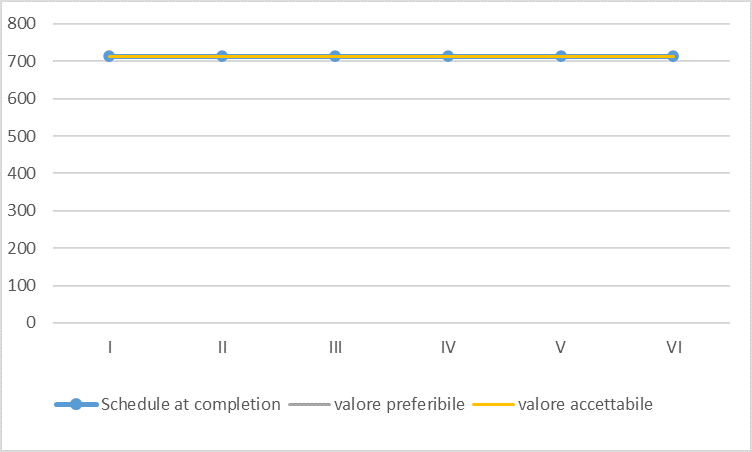
\includegraphics[width=\linewidth]{./img/grafici/RQ13.png}	
	\caption{M13 revisione di qualifica}	
\end{figure}
\begin{itemize}
	\item \textbf{Valore preferibile}: pari a quanto preventivato;
	\item \textbf{Valore accettabile}: pari a quanto preventivato;
	\item \textbf{Considerazioni}: la metrica\glosp risulta soddisfatta al termine del periodo di qualifica.
\end{itemize}

\subparagraph{M14 Rischi non preventivati} \mbox{}
\begin{longtable}[H!] {						
		>{}p{50mm}  		
		>{}p{8mm}
		>{}p{8mm}		
		>{}p{8mm}		
		>{}p{8mm}		
		>{}p{8mm}		
		>{}p{8mm}
		>{}p{8mm}
		>{}p{8mm}
		>{}p{8mm}
	}
	\rowcolor{gray!50}
	\textbf{} & \textbf{I} & \textbf{II} & \textbf{III} & \textbf{IV} & \textbf{V} & \textbf{VI} \TBstrut \\ [2mm]
	\textbf{Numero di rischi} & 0 & 0 & 0 & 0 & 0 & 0 \TBstrut \\ [2mm]
	\rowcolor{white}
	\caption{M14 revisione di qualifica}
\end{longtable}
\begin{figure}[H] 	
	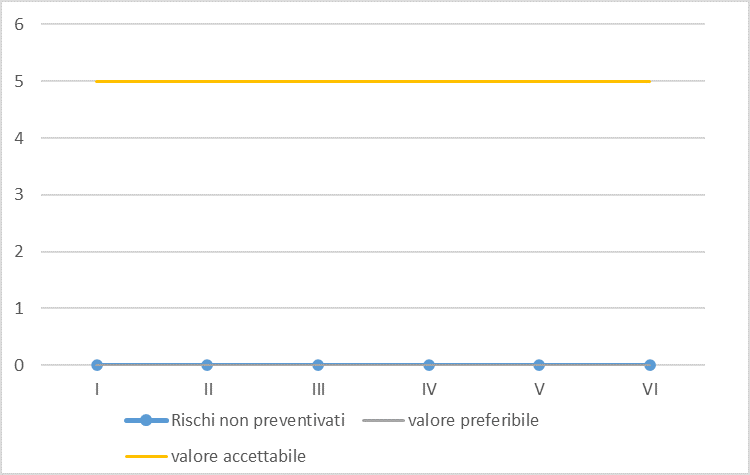
\includegraphics[width=\linewidth]{./img/grafici/RQ14.png}	
	\caption{M14 revisione di qualifica}	
\end{figure}
\begin{itemize}
	\item \textbf{Valore preferibile}: $=0$;
	\item \textbf{Valore accettabile}: $\le 5$;
	\item \textbf{Considerazioni}: la metrica\glosp risulta soddisfatta al termine del periodo di qualifica.
\end{itemize}

\paragraph{Qualità di prodotto}

\paragraph*{PRD-Q1 Documenti}
\paragraph{M19 Correttezza ortografica} \mbox{}
\begin{longtable}[H!] {						
		>{}p{50mm}  		
		>{}p{8mm}
		>{}p{8mm}		
		>{}p{8mm}		
		>{}p{8mm}		
		>{}p{8mm}		
		>{}p{8mm}
		>{}p{8mm}
		>{}p{8mm}
		>{}p{8mm}
	}
	\rowcolor{gray!50}
	\textbf{} & \textbf{I} & \textbf{II} & \textbf{III} & \textbf{IV} & \textbf{V} & \textbf{VI} \TBstrut \\ [2mm]
	\textbf{Numero errori} & 0 & 1 & 0 & 0 & 0 & 0 \TBstrut \\ [2mm]
	\rowcolor{white}
	\caption{M19 revisione di qualifica}
\end{longtable}
\begin{figure}[H] 	
	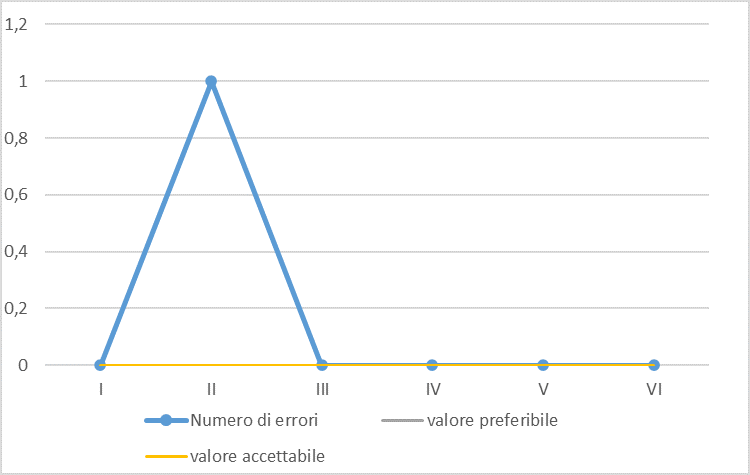
\includegraphics[width=\linewidth]{./img/grafici/RQ19.png}	
	\caption{M19 revisione di qualifica}	
\end{figure}
\begin{itemize}
	\item \textbf{Valore preferibile}: 0;
	\item \textbf{Valore accettabile}: 0;
	\item \textbf{Considerazioni}: la metrica\glosp risulta soddisfatta al termine del periodo di qualifica.
\end{itemize}


\paragraph*{PRD-Q2 Appropriatezza funzionale}
\subparagraph{M16 Percentuale requisiti obbligatori soddisfatti} \mbox{}
\begin{longtable}[H!] {						
		>{}p{50mm}  		
		>{}p{8mm}
		>{}p{8mm}		
		>{}p{8mm}		
		>{}p{8mm}		
		>{}p{8mm}		
		>{}p{8mm}
		>{}p{8mm}
		>{}p{8mm}
		>{}p{8mm}
	}
	\rowcolor{gray!50}
	\textbf{} & \textbf{I} & \textbf{II} & \textbf{III} & \textbf{IV} & \textbf{V} & \textbf{VI} \TBstrut \\ [2mm]
	\textbf{Percentuale} & 55\% & 58\% & 61\% & 68\% & 77\% & 87\% \TBstrut \\ [2mm]
	\rowcolor{white}
	\caption{M16 revisione di qualifica}
\end{longtable}
\begin{figure}[H] 	
	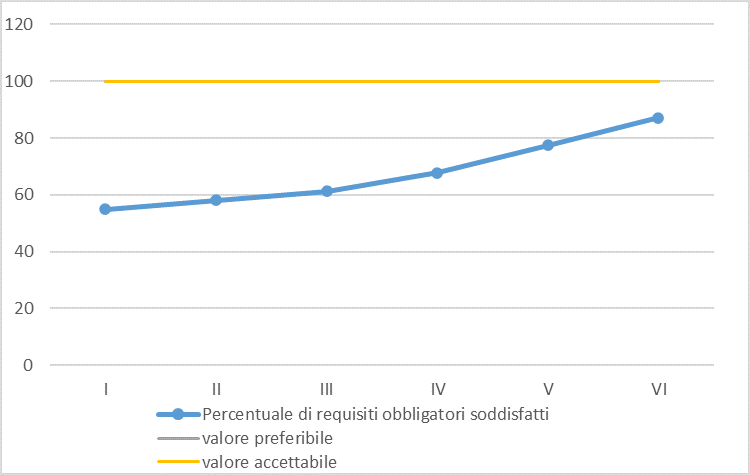
\includegraphics[width=\linewidth]{./img/grafici/RQ16.png}	
	\caption{M16 revisione di qualifica}	
\end{figure}
\begin{itemize}
	\item \textbf{Valore preferibile}: $=100\%$;
	\item \textbf{Valore accettabile}: $=100\%$;
	\item \textbf{Considerazioni}: la metrica\glosp risulta non soddisfatta al termine del periodo di qualifica.
\end{itemize}

\subparagraph{M17 Percentuale requisiti desiderabili soddisfatti} \mbox{}
\begin{longtable}[H!] {						
		>{}p{50mm}  		
		>{}p{8mm}
		>{}p{8mm}		
		>{}p{8mm}		
		>{}p{8mm}		
		>{}p{8mm}		
		>{}p{8mm}
		>{}p{8mm}
		>{}p{8mm}
		>{}p{8mm}
	}
	\rowcolor{gray!50}
	\textbf{} & \textbf{I} & \textbf{II} & \textbf{III} & \textbf{IV} & \textbf{V} & \textbf{VI} \TBstrut \\ [2mm]
	\textbf{Percentuale} & 9\% & 9\% & 9\% & 9\% & 9\% & 9\% \TBstrut \\ [2mm]
	\rowcolor{white}
	\caption{M17 revisione di qualifica}
\end{longtable}
\begin{figure}[H] 	
	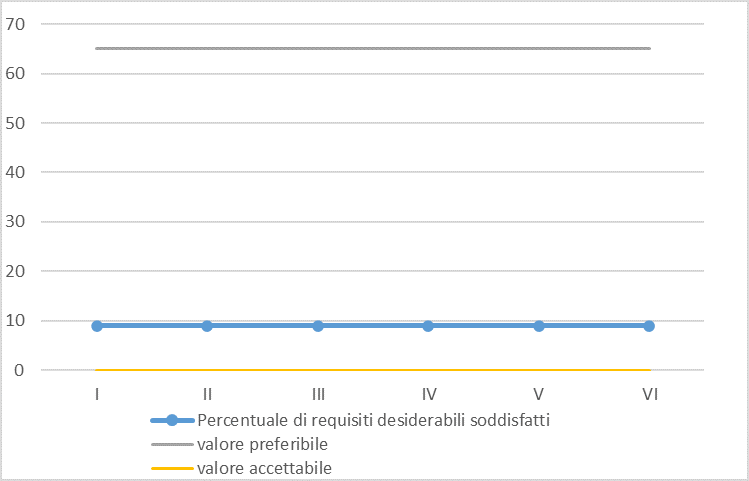
\includegraphics[width=\linewidth]{./img/grafici/RQ17.png}	
	\caption{M17 revisione di qualifica}	
\end{figure}
\begin{itemize}
	\item \textbf{Valore preferibile}: $\ge 65\%$;
	\item \textbf{Valore accettabile}: $\ge 0\%$;
	\item \textbf{Considerazioni}: la metrica\glosp risulta soddisfatta al termine del periodo di qualifica.
\end{itemize}

\subparagraph{M18 Percentuale requisiti opzionali soddisfatti} \mbox{}
\begin{longtable}[H!] {						
		>{}p{50mm}  		
		>{}p{8mm}
		>{}p{8mm}		
		>{}p{8mm}		
		>{}p{8mm}		
		>{}p{8mm}		
		>{}p{8mm}
		>{}p{8mm}
		>{}p{8mm}
		>{}p{8mm}
	}
	\rowcolor{gray!50}
	\textbf{} & \textbf{I} & \textbf{II} & \textbf{III} & \textbf{IV} & \textbf{V} & \textbf{VI} \TBstrut \\ [2mm]
	\textbf{Percentuale} & 0\% & 0\% & 0\% & 0\% & 0\% & 0\% \TBstrut \\ [2mm]
	\rowcolor{white}
	\caption{M18 revisione di qualifica}
\end{longtable}
\begin{figure}[H] 	
	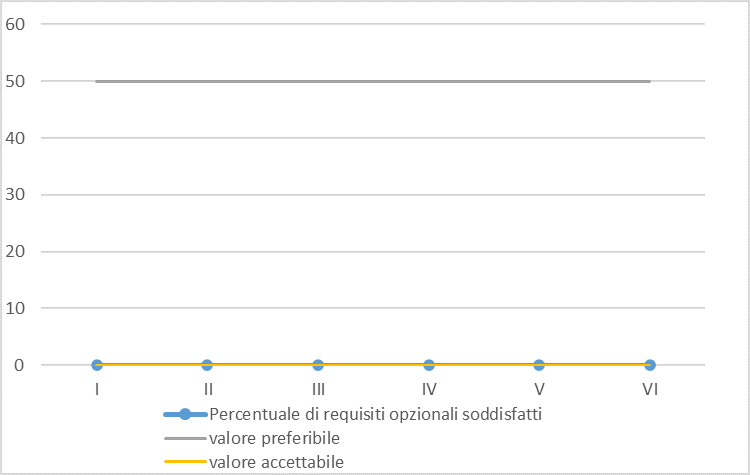
\includegraphics[width=\linewidth]{./img/grafici/RQ18.png}	
	\caption{M18 revisione di qualifica}	
\end{figure}
\begin{itemize}
	\item \textbf{Valore preferibile}: $\ge 50\%$;
	\item \textbf{Valore accettabile}: $\ge 0\%$;
	\item \textbf{Considerazioni}: la metrica\glosp risulta soddisfatta al termine del periodo di qualifica.
\end{itemize}

\subparagraph{M26 Percentuale test passati} \mbox{}
\begin{longtable}[H!] {						
		>{}p{50mm}  		
		>{}p{8mm}
		>{}p{8mm}		
		>{}p{8mm}		
		>{}p{8mm}		
		>{}p{8mm}		
		>{}p{8mm}
		>{}p{8mm}
		>{}p{8mm}
		>{}p{8mm}
	}
	\rowcolor{gray!50}
	\textbf{} & \textbf{I} & \textbf{II} & \textbf{III} & \textbf{IV} & \textbf{V} & \textbf{VI} \TBstrut \\ [2mm]
	\textbf{Percentuale} & 83\% & 100\% & 79\% & 98\% & 100\% & 100\% \TBstrut \\ [2mm]
	\rowcolor{white}
	\caption{M26 revisione di qualifica}
\end{longtable}
\begin{figure}[H] 	
	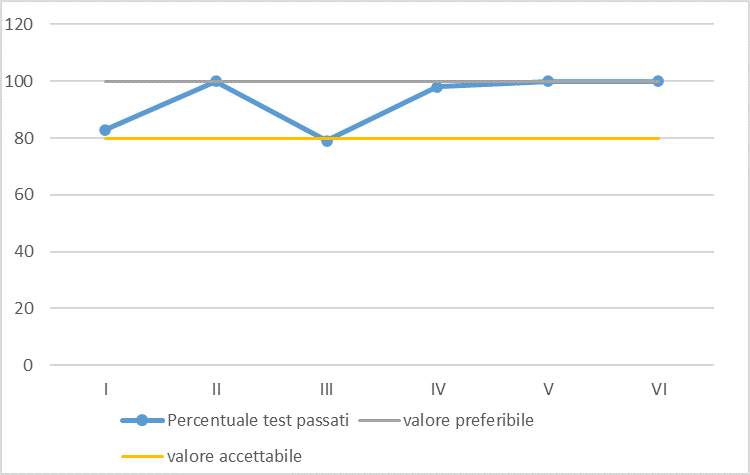
\includegraphics[width=\linewidth]{./img/grafici/RQ26.png}	
	\caption{M26 revisione di qualifica}	
\end{figure}
\begin{itemize}
	\item \textbf{Valore preferibile}: $= 100\%$;
	\item \textbf{Valore accettabile}: $\ge 80\%$;
	\item \textbf{Considerazioni}: la metrica\glosp risulta soddisfatta al termine del periodo di qualifica.
\end{itemize}











%\paragraph{M27 Structural fan out} \mbox{}
%\begin{longtable}[H!] {						
%		>{}p{50mm}  		
%		>{}p{8mm}
%		>{}p{8mm}		
%		>{}p{8mm}		
%		>{}p{8mm}		
%		>{}p{8mm}		
%		>{}p{8mm}
%		>{}p{8mm}
%		>{}p{8mm}
%		>{}p{8mm}
%	}
%	\rowcolor{gray!50}
%	\textbf{} & \textbf{I} & \textbf{II} & \textbf{III} & \textbf{IV} & \textbf{V} & \textbf{VI} \TBstrut \\ [2mm]
%	\textbf{Numero} & 4 & 6 & 6 & 6 & 6 & 6 \TBstrut \\ [2mm]
%	\rowcolor{white}
%	\caption{M27 revisione di qualifica}
%\end{longtable}
%\begin{figure}[H] 	
%	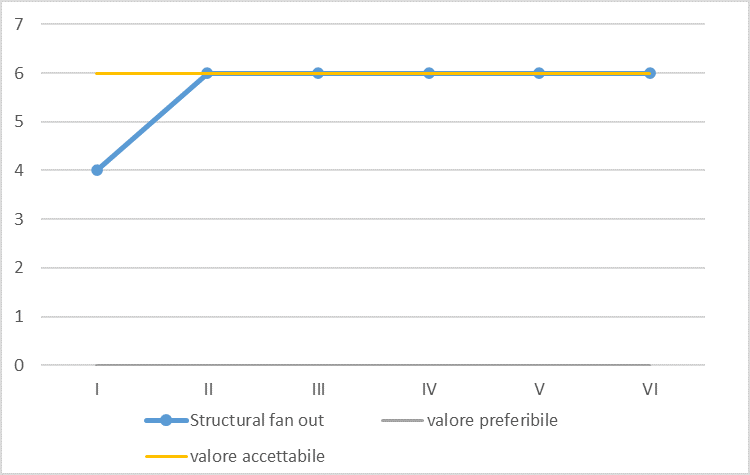
\includegraphics[width=\linewidth]{./img/grafici/RQ27.png}	
%	\caption{M27 revisione di qualifica}	
%\end{figure}
%\begin{itemize}
%	\item \textbf{Valore preferibile}: $0$
%	\item \textbf{Valore accettabile}: $ \le 6$
%	\item \textbf{Considerazioni}: la metrica\glosp risulta soddisfatta al termine del periodo di qualifica.
%\end{itemize}
